\chapter{COLORING FROM ALMOST DEGREE SIZED PALETTES}
\label{ListColoringChapter}
\begin{center}
\emph{The material in this chapter appeared in \cite{mules} and is joint work with Dan Cranston.}
\end{center}

In this section we use list-coloring lemmas to forbid a large class of graphs
from appearing as induced subgraphs of vertex critical graphs satisfying $\chi = \Delta$.  In each case, we assume that such a graph
$H\lhd G$ appears as an induced subgraph of such a graph $G$.  By criticality of
$G$, we can color $G\setminus H$ with $\Delta-1$ colors.  If $H$ can be colored
regardless of which colors are forbidden by its colored neighbors in $G\setminus
H$, then we can clearly extend this coloring to all of $G$.  Such $H$ are precisely the $d_1$-choosable graphs.

We characterize all graphs $\join{A}{B}$ with $|A|\ge 2$,
$|B|\ge 2$ that are not $d_1$-choosable.
The characterization is somewhat lengthy, so we split it into a number of
lemmas.  For the case $|A|\ge 4$, $|B|\ge 4$, see
Lemma~\ref{BothSidesAtLeastFourD1Choose}.  When $|A|= 3$, we consider the
four cases $A=E_3$ (Lemma~\ref{E3Classification}), $A=\overline{P_3}$
(Lemma~\ref{AntiP3Classification}), $A=P_3$ (Lemma~\ref{P3Classification}), and
$A=K_3$ (Lemma~\ref{ConnectedEqual3Poss}).
When $|A|=2$, we consider the case $A=E_2$ in
Lemma~\ref{E2Classification} and the case $A=K_2$ in Lemma~\ref{K2Classification}.

\smallskip

Let $G$ be a graph.  A \emph{list assignment} to the vertices of $G$ is a
function from $V(G)$ to the finite subsets of $\mathbb{N}$.  A list assignment
$L$ to $G$ is \emph{good} if $G$ has a coloring $c$ where $c(v) \in L(v)$ for
each $v \in V(G)$.  It is \emph{bad} otherwise.  We call the collection of all
colors that appear in $L$, the \emph{pot} of $L$.  That is $Pot(L) \DefinedAs
\bigcup_{v \in V(G)} L(v)$.  For a subgraph $H$ of $G$ we write $Pot_H(L)
\DefinedAs \bigcup_{v \in V(H)} L(v)$. For $S \subseteq Pot(L)$, let $G_S$ be
the graph $G\left[\setb{v}{V(G)}{L(v) \cap S \neq \emptyset}\right]$.  We also
write $G_c$ for $G_{\{c\}}$. We let $\fancy{B}(L)$ be the bipartite graph that
has parts $V(G)$ and $Pot(L)$ and an edge from $v \in V(G)$ to $c \in Pot(L)$
iff $c \in L(v)$. For $\func{f}{V(G)}{\IN}$, an $f$-assignment on $G$ is an
assignment $L$ of lists to the vertices of $G$ such that $\card{L(v)} = f(v)$
for each $v \in V(G)$.  We say that $G$ is \textit{$f$-choosable} if every
$f$-assignment on $G$ is good.

\section{Shrinking the pot}
In this section we prove a lemma about bad list assignments with minimum pot size.  
Some form of this lemma has appeared independently in at least two places we know of---Kierstead \cite{kierstead2000choosability} and Reed and Sudakov \cite{ReedSudakov}.  
We will use this lemma repeatedly in the arguments that follow.

Given a graph $G$ and $\func{f}{V(G)}{\mathbb{N}}$, we have a partial order on the $f$-assignments to $G$ given by $L < L'$ iff $\card{Pot(L)} < \card{Pot(L')}$.  When we talk of \emph{minimal} $f$-assignments, we mean minimal with respect to this partial order.

\begin{lem}\label{CannotColorSelfWithSelf}
Let $G$ be a graph and $\func{f}{V(G)}{\mathbb{N}}$.  Assume $G$ is not $f$-choosable and let $L$ be a minimal bad $f$-assignment. Assume $L(v) \neq Pot(L)$ for each $v \in V(G)$.  Then, for each nonempty $S \subseteq Pot(L)$, any coloring of $G_S$ from $L$ uses some color not in $S$.
\end{lem}
\begin{proof}
Suppose not and let $\emptyset \neq S \subseteq Pot(L)$ be such that $G_S$ has a coloring $\phi$ from $L$ using only colors in $S$.  For $v \in V(G)$, let $h(v)$ be the smallest element of $Pot(L) - L(v)$ (this is well defined by assumption). Pick some $c \in S$ and construct a new list assignment $L'$ as follows.

\[L'(v) = \left \{ \begin{array}{rl}
L(v) &\mbox{ if $v \in V(G) - V(G_S)$} \\
L(v) &\mbox{ if $v \in V(G_S)$ and $c \not \in L(v)$} \\
\left(L(v) - \{c\}\right) \cup \{h(v)\} &\mbox{ if $v \in V(G_S)$ and $c\in L(v)$} \\
\end{array} \right.\]

Note that $L'$ is an $f$-assignment and $Pot(L') = Pot(L) - \{c\}$.  Thus, by minimality of $L$, we can properly color $G$ from $L'$.  In particular, we have a coloring of $V(G) - V(G_S)$ from $L$ using no color from $S$.  We can complete this to a coloring of $G$ from $L$ using $\phi$. This contradicts the fact that $L$ is bad.  
\end{proof}

When $|S| = 1$, we can say more.  We will use the following lemma in the proof
that the graph $D_8$ in Figure \ref{fig:D8} is $d_1$-choosable.  It should be
useful elsewhere as well.

\begin{lem}\label{ComponentsOfColor}
Let $G$ be a graph and $\func{f}{V(G)}{\mathbb{N}}$.  
Suppose $G$ is not $f$-choosable and let $L$ be a minimal bad $f$-assignment.
Then for any $c \in Pot(L)$, there is a component $H$ of $G_c$ such that
$Pot_H(L) = Pot(L)$.  In particular, $Pot_{G_c}(L) = Pot(L)$.
\end{lem}
\begin{proof}
Suppose otherwise that we have $c \in Pot(L)$ such that $Pot_H(L) \subsetneq
Pot(L)$ for all components $H$ of $G_c$.  Say the components of $G_c$ are
$H_1, \ldots, H_t$. For $i \in \irange{t}$, choose $\alpha_i \in Pot(L) -
Pot_{H_i}(L)$. Now define a list assignment $L'$ on $G$ by setting $L'(v)
\DefinedAs L(v)$ for all $v \in V(G) - V(G_c)$ and for each $i \in \irange{t}$
setting $L'(v) \DefinedAs (L(v) - c) \cup \set{\alpha_i}$ for each $v \in
V(H_i)$.  Then $\card{Pot(L')} < \card{Pot(L)}$ and hence by minimality $L$ we
have an $L'$-coloring $\pi$ of $G$.  Plainly $Q \DefinedAs
\setb{v}{V(G_c)}{\pi(v) = \alpha_i \text{ for some $i \in \irange{t}$}}$ is an
independent set.  Since $c$ doesn't appear outside $G_c$, we can recolor
all vertices in $Q$ with $c$ to get an $L$-coloring of $G$.  This contradicts
the fact that $L$ is bad.
\end{proof}

\begin{defn}
A bipartite graph with parts $A$ and $B$ has \emph{positive surplus} (with respect to $A$) if $\card{N(X)} > \card{X}$ for all $\emptyset \neq X \subseteq A$.
\end{defn}

\begin{lem}\label{MinPotCondition}
Let $G$ be a graph and $\func{f}{V(G)}{\mathbb{N}}$.  Assume $G$ is not $f$-choosable and let $L$ be a minimal bad $f$-assignment. Assume $L(v) \neq Pot(L)$ for each $v \in V(G)$. Then $\fancy{B}(L)$ has positive surplus (with respect to $Pot(L)$).
\end{lem}
\begin{proof}
Suppose not and choose $\emptyset \neq X \subseteq Pot(L)$ such that $\card{N(X)} \leq \card{X}$ minimizing $\card{X}$. If $\card{X} = 1$, then $G_X$ can be colored from $X$ contradicting Lemma \ref{CannotColorSelfWithSelf}.  Hence $\card{X} \geq 2$.  By minimality of $\card{X}$, for any $Y \subset X$,
$\card{N(Y)} \geq \card{Y} + 1$.  Hence, for any $x \in X$, we have $\card{N(X)} \geq \card{N(X - \set{x})} \geq \card{X - \set{x}} + 1 = \card{X}$.  Thus, by Hall's Theorem, we have a matching of $X$ into $N(X)$, but $\card{N(X)} \leq \card{X}$ so this gives a coloring of $G_X$ from $X$ contradicting Lemma \ref{CannotColorSelfWithSelf}.
\end{proof}

Our approach to coloring a graph (particularly a join) will often be to
consider nonadjacent vertices $u$ and $v$ and show that their lists contain a
common color.  By the pigeonhole principle, this follows immediately when
$|L(u)|+|L(v)|>|Pot(L)|$.  We will use the following lemma frequently throughout
the remainder of this paper.

\begin{SmallPotLemma}
Let $G$ be a graph and $\func{f}{V(G)}{\mathbb{N}}$ with $f(v) < \card{G}$ for all $v \in V(G)$.  If $G$ is not $f$-choosable, then $G$ has a minimal bad $f$-assignment $L$ such that $\card{Pot(L)} < \card{G}$.
\end{SmallPotLemma}
\begin{proof}
Suppose not and let $L$ be a minimal bad $f$-assignment. For each $v \in V(G)$ we have $\card{L(v)} = f(v) < \card{G} \leq \card{Pot(L)}$ and hence $L(v) \neq Pot(L)$.  Thus by Lemma \ref{MinPotCondition} we have the contradiction $\card{G} \geq \card{N(Pot(L))} > \card{Pot(L)}$.
\end{proof}

\section{Degree choosability}
\label{Degree choosability}
\begin{defn}
Let $G$ be a graph and $r \in \mathbb{Z}$.  Then $G$ is \emph{$d_r$-choosable} if $G$ is $f$-choosable where $f(v) = d(v) - r$.
\end{defn}

Note that a vertex critical graph with $\chi = \Delta + 1 - r$ contains no
induced $d_r$-choosable subgraph.  Since we are working to prove the
Borodin-Kostochka conjecture, we will focus on the case $r=1$ and primarily
study $d_1$-choosable graphs.  For $r=0$, we have the following well known generalization of Brooks' Theorem due independently to Borodin \cite{borodin1977criterion} and Erd\H{o}s, Rubin and Taylor \cite{erdos1979choosability}. 

\subsection{Degree-choosable graphs}
\begin{defn}
A \emph{Gallai tree} is a graph all of whose blocks are complete graphs or odd cycles.
\end{defn}

\begin{ClassificationOfd0}
For any connected graph $G$, the following are equivalent.
\begin{itemize}
\item $G$ is $d_0$-choosable.
\item $G$ is not a Gallai tree.
\item $G$ contains an induced even cycle with at most one chord.
\end{itemize}
\end{ClassificationOfd0}

In \cite{BrooksExtended}, Kostochka, Stiebitz and Wirth give a short proof of the equivalence of (1) and (2) as well as extending the result to hypergraphs.  In \cite{Hladky}, Hladk{\`y}, Kr{\'a}l and Schauz gave an algebraic proof (Rubin's block theorem below plus the Alon-Tarsi theorem \cite{Alon1992125}), it also works for paintability (online list-choosability), see \cite{schauz2009mr}.

We give some lemmas about $d_0$-assignments that will be useful in the later study of general $d_k$-assignments.  Combined with the following structural result, these lemmas give a quick proof of the classification of $d_0$-choosable graphs. The following lemma from \cite{erdos1979choosability} is due to Rubin.  For other proofs, see \cite{Entringer1985367} and \cite{Hladky}.

\begin{lem}\label{gallaitreeevencycle}
Any $2$-connected graph is complete, an odd cycle or contains an induced even cycle with at most one chord.
\end{lem}
\begin{proof}
Suppose not and choose a counterexample $G$ minimizing $\card{G}$. Since $G$ is
$2$-connected and not complete, it contains an induced cycle $C$ of length at
least four. Then $C$ is an induced odd cycle and thus $G-C$ is not empty.  Since
$G$ is $2$-connected, we may choose a shortest $C$-path in $G$ with distinct ends in $C$---call it $R$.  Since $G[V(C) \cup V(R)]$ is $2$-connected, by minimality of $\card{G}$, $V(G) = V(C) \cup V(R)$.

First suppose $R$ has length at least $3$.  Then since $R$ is shortest, $G = C \cup R$ and thus one of the small cycles in $C \cup R$ is an even induced cycle or the large cycle is an even induced cycle with at most one chord, giving a contradiction.

Thus $R$ has length $2$.  Let $z$ be the vertex on $R$ in $G-C$.  If $z$ has only two neighbors in $C$, then we get a contradiction as in the previous paragraph.  Thus $z$ has at least three neighbors $a,b,c \in V(C)$.  Now $\card{C} \geq 4$ since $G$ is not complete.  Thus, without loss of generality, the vertices between $a$ and $b$ on $C$ in cyclic order are $w_1, \ldots, w_k$ with $k \geq 1$.  But $G - \set{w_1,\ldots, w_k}$ is $2$-connected, not complete, and not an odd cycle.  Hence, by minimality of $\card{G}$, $G - \set{w_1,\ldots, w_k}$ contains an induced even cycle with at most one chord.  This final contradiction completes the proof.
\end{proof}

The following lemma was used in \cite{BrooksExtended}.
\begin{lem}\label{d0Subgraph}
A connected graph is $d_0$-choosable iff it contains a $d_0$-choosable induced subgraph. 
\end{lem}
\begin{proof}
The forward direction is plain.  For the reverse, let $H \unlhd G$ be $d_0$-choosable.  Since $G$ is connected, we can order $V(G)$ such that each vertex in $V(G - H)$ has a neighbor after it and $V(H)$ comes last.  Coloring $V(G-H)$ greedily from the lists in this order leaves a $d_0$-assignment on $H$ which we can complete by assumption.
\end{proof}

\begin{lem}\label{d0NeighborList}
Let $L$ be a bad $d_0$-assignment on a connected graph $G$ and $x \in V(G)$ a noncutvertex. Then $L(x) \subseteq L(y)$ for each $y \in N(x)$.
\end{lem}
\begin{proof}
Suppose otherwise that we have $c \in L(x) - L(y)$ for some $y \in N(x)$.  Coloring $x$ with $c$ leaves at worst a $d_0$-assignment $L'$ on the connected $H \DefinedAs G-x$ where $\card{L'(y)} > d_H(y)$.  But then we can complete the coloring, a contradiction.
\end{proof}

\begin{lem}\label{d0Subdivision}
Any even subdivision of a bridgeless $d_0$-choosable graph is $d_0$-choosable.
\end{lem}
\begin{proof}
Since subdividing an edge cannot create a bridge, it suffices to show that subdividing an edge with two vertices preserves $d_0$-choosability.  Let $G$ be a bridgeless $d_0$-choosable graph.  Suppose there exists $xy \in E(G)$ such that subdividing $xy$ with vertices $w$ and $z$ creates a graph $H$ which is not $d_0$-choosable.  Let $L$ be a bad $d_0$-assignment on $H$.  Since $G$ is bridgeless, $w$ and $z$ are not cutvertices of $H$.  By Lemma \ref{d0NeighborList}, $L(w) = L(z)$.  But $L$ restricted to $G$ is a $d_0$-assignment, so we have a coloring $\pi$ of $H - \set{w, z}$ from $L$ such that $\pi(x) \neq \pi(y)$.  Now $L(w) - \set{\pi(x)} \neq L(z) - \set{\pi(y)}$ so we can complete the coloring to all of $H$, a contradiction.
\end{proof}

Using the Small Pot Lemma it is easy to prove that $C_4$ and $K_4^-$ are $d_0$-choosable which combined with Lemma \ref{d0Subdivision} shows that every even cycle with at most one chord is $d_0$-choosable.  It turns out that the conclusion of the Small Pot Lemma holds for general bad $d_0$-assignments, not just minimal ones.  We will use the following lemma often in proofs when we end up with a bad $d_0$-assignment that may not be minimal.

\begin{lem}\label{d0PotColoring}
If $L$ a bad $d_0$-assignment on a connected graph $G$, $\card{Pot(L)} < \card{G}$.
\end{lem}
\begin{proof}
Suppose that the lemma is false and choose a connected graph $G$ together with a bad $d_0$-assignment $L$ where $\card{Pot(L)} \geq \card{G}$ minimizing $\card{G}$.  Plainly, $\card{G} \geq 2$.  Let $x \in G$ be a noncutvertex (any end block has at least one).  By Lemma \ref{d0NeighborList}, $L(x) \subseteq L(y)$ for each $y \in N(x)$. Thus coloring $x$ decreases the pot by at most one, giving a smaller counterexample.  This contradiction completes the proof.
\end{proof}

\begin{proof}[Proof of the classification of $d_0$-choosable graphs]
It is easy to construct a bad $d_0$-assignment on a Gallai tree---hence (1) implies (2).  Now if a graph is not a Gallai tree, then some block is neither complete nor an odd cycle.  But then, by Lemma \ref{gallaitreeevencycle}, that block contains an induced even cycle with at most one chord.  Hence (2) implies (3).  

Now we prove that $C_4$ and $K_4^-$ are $d_0$-choosable.  If not, then we have a bad $d_0$-assignment $L$ on $C_4$ or $K_4^-$.  By Lemma \ref{d0PotColoring}, $\card{Pot(L)} \leq 3$.  Hence some nonadjacent pair can be colored the same leaving a $d_{-1}$-assignment on the components which can be easily completed.

Thus, by Lemma \ref{d0Subdivision}, any even cycle with at most one chord is $d_0$-choosable.  Combining this with Lemma \ref{d0Subgraph} proves that (3) implies (1).
\end{proof}

\subsection{Basic properties}
We also need a few basic lemmas about how $d_r$-choosability behaves with respect to induced subgraphs.

\begin{lem}\label{PartialdkLemma}
Fix $r \geq 0$. Let $G$ be a graph and $H \unlhd G$ a $d_r$-choosable subgaph. If $L$ is a $d_r$-assignment on $G$ and $G - H$ is properly colorable from $L$, then $G$ is properly colorable from $L$.
\end{lem}
\begin{proof}
Color $G - H$ from $L$. Let $L'$ be the resulting list assignment on $H$.  Since each $v \in V(H)$ must be adjacent to as many vertices as colors in $G - H$ we see that $L'$ is again a $d_r$-assignment.  The lemma follows.
\end{proof}

\begin{lem}\label{ColorableSubgraphdk}
Fix $r \geq 0$. Let $G$ be a graph and $H \unlhd G$ a $d_r$-choosable subgaph.  If there exists an ordering $v_1, \ldots, v_t$ of the vertices of $G - H$
such that $v_i$ has degree at least $r+1$ in $G[V(H) \cup \bigcup_{1 \leq j \leq i - 1} v_j]$ for each $i$, then $G$ is $d_r$-choosable.
\end{lem}
\begin{proof}
Let $L$ be a $d_r$-assignment on $G$. Go through $G-H$ in order $v_t, \ldots, v_1$ coloring $v_i$ with the smallest available color in $L(v_i)$.  Since when we go to color $v_i$, it has at least $r+1$ uncolored neighbors we succeed in coloring $G-H$.  Now the lemma follows from Lemma \ref{PartialdkLemma}.
\end{proof}

We will also use the following immediate consequence of the pigeonhole principle.

\begin{lem}\label{BasicFiniteSets}
If $S_1, \ldots, S_m$ are nonempty subsets of a finite set $T$ and $\sum_{i \geq 1} \card{S_i} > (m - 1)\card{T}$, then $\bigcap_{i \geq 1} S_i \neq \emptyset$.
\end{lem}


\section{Handling joins}
The main result of this section is Lemma~\ref{ConnectedJoin}, which
plays a key role in our classification of bad graphs $A*B$.  Specifically,
Lemma~\ref{ConnectedJoin} is essential to the proof of
Lemma~\ref{ConnectedAtLeast4Poss}, which considers the case when $|A|\ge 4$ and
$B$ is arbitrary.

\begin{lem}\label{ArbitrarySubgraphLemma}
Fix $r \geq 0$. Let $A$ be a graph with $\card{A} \geq r + 1$ and $B$ a nonempty graph.  If $\join{A}{B}$ is $d_r$-choosable, then $\join{A}{C}$ is 
$d_r$-choosable for any graph $C$ with $B \unlhd C$.
\end{lem}
\begin{proof}
Assume $\join{A}{B}$ is $d_r$-choosable and let $C$ be a graph with $B \unlhd C$.  Put $H = C - B$.  For each $v \in V(H)$, 
$\card{L(v)} \geq d(v) - r \geq d_H(v) + r + 1 - r = d_H(v) + 1$.  Thus we may color $H$ from its lists.  By Lemma \ref{PartialdkLemma}, we can complete the coloring to all of $\join{A}{C}$.
\end{proof}

\begin{lem}\label{ConnectedSubgraphLemma}
Fix $r \geq 0$. Let $A$ be a graph with $\card{A} \geq r$ and $B$ a nonempty graph.  If $\join{A}{B}$ is $d_r$-choosable, then $\join{A}{C}$ is 
$d_r$-choosable for any connected graph $C$ with $B \unlhd C$.
\end{lem}
\begin{proof}
Assume $\join{A}{B}$ is $d_r$-choosable and let $C$ be a connected graph with $B \unlhd C$.  Put $H = C - B$.  For each $v \in H$, $\card{L(v)} \geq d(v) - r \geq d_H(v) + r - r = d_H(v)$.  Since $C$ is connected, each component of $H$ has a vertex $v$ that hits a vertex in $B$ and hence has $\card{L(v)} \geq d_H(v) + 1$. Thus we may color $H$ from its lists.  By 
Lemma \ref{PartialdkLemma}, we can complete the coloring to all of $\join{A}{C}$.
\end{proof}

\begin{lem}\label{E2bringsdown}
Fix $r \geq 0$.  Let $G$ be a $d_{r - 1}$ choosable graph with at least $2r + 2$ vertices. Then $\join{E_2}{G}$ is $d_r$-choosable.
\end{lem}
\begin{proof}
Let $x,y$ be the vertices in the $E_2$.  Suppose $E_2*G$ is not $d_r$-choosable.  Then by the Small Pot Lemma,
we have a $d_r$-assignment $L$ with $\card{Pot(L)} < 2 + \card{G}$. 
Now $\card{L(x)} + \card{L(y)} \geq d(x) + d(y) - 2r \geq 2\card{G} - 2r \geq 2
+ \card{G} > |Pot(L)|$, since $\card{G} \geq 2r+2$.  Thus we can use a single common color
on $x$ and $y$, leaving a $d_{r-1}$-assignment on $G$.  We may now complete the coloring, giving a contradiction.
\end{proof}

Since every graph is $d_{-1}$-choosable we get the following immediately.
\begin{cor}\label{E2rJoinK2}
For $r \geq 0$, both $E_2^{r+2}$ and $\join{E_2^{r+1}}{K_2}$ are $d_r$-choosable.
\end{cor}

Note that this is equivalent to the following fundamental result of Erd\H{o}s, Rubin and Taylor \cite{erdos1979choosability}. 

\begin{lem}\label{E2n}
For all $n \geq 1$, $E_2^n$ is $n$-choosable.
\end{lem}

\begin{lem}\label{ArbitraryJoin}
Fix $r \geq 0$.  Let $A$ be a graph with $\card{A} \geq 3r+2$ and $B$ an arbitrary graph.  If $\join{A}{B}$ is not $d_r$-choosable, then
$\omega(B) \geq \card{B} - 2r$.
\end{lem}
\begin{proof}
Suppose $G \DefinedAs \join{A}{B}$ is not $d_r$-choosable and let $L$ be a minimal bad $d_r$-assignment. Then, by the Small Pot Lemma, $\card{Pot(L)} \leq \card{G} - 1$.  Let $\func{g}{S}{Pot_S(L)}$ be a partial coloring of $B$ from $L$ maximizing $\card{S} - \card{im(g)}$ and then minimizing $\card{S}$.  Color $S$ using $g$ and let $L'$ be the resulting list assignment.

Put $H \DefinedAs G - S$ and $C \DefinedAs B - S$. 
First suppose that $\card{S}- \card{im(g)} \geq r+1$. 
For each $v \in C$ we have $\card{L'(v)} \geq d_C(v) - r + 3r+2 > d_C(v)$, so we
can complete $g$ to $C$.
This leaves each $v \in V(A)$ with a list of size at least $d_A(v) - r +
\card{S} - \card{im(g)} > d_A(v)$.  Hence, we can complete the coloring to all
of $G$.  Thus $L$ is not bad after all, giving a contradiction.  

So instead we assume that $|S|-|im(g)|\le r$.
By the minimality condition on $\card{S}$ we see that $g$ has
no singleton color classes.  In particular, $\card{S} \geq 2\card{im(g)}$.  By
combining this inequality with $|S|-|im(g)|\le r$, we get $\card{S} \leq 2r$.
Since $|C|=|B|-|S|\ge |B|-2r$, the conclusion will follow if we can show that $C$ is complete.

By definition, $\card{Pot(L')} = \card{Pot(L)} - \card{im(g)}$.
By the maximality condition on $g$, every pair of nonadjacent vertices in $C$
must have disjoint lists under $L'$ (otherwise we could use a common color on
nonadjacent vertices in $C$ and increase $|S|-|im(g)|$).  
Let $I$ be a maximal independent set in $C$.  To reach a contradiction, we assume
that $\card{I} \geq 2$.
Then for all the elements of $I$ to have disjoint lists, we must have
\begin{align*}
 \sum_{v \in I} \card{L'(v)} &\leq \card{Pot(L')} \\
 \sum_{v \in I} (d_H(v) - r) &\leq \card{Pot(L')} \\
 \sum_{v \in I} (\card{A} + d_C(v) - r) &\leq \card{Pot(L')} \\
 (\card{A}-r)\card{I} + \sum_{v \in I} d_C(v) &\leq \card{Pot(L')} \\
 (\card{A}-r)\card{I} + \card{C} - \card{I} &\leq \card{Pot(L')} \\
 (\card{A} - r - 1)\card{I} + \card{B}- \card{S}&\leq \card{A} + \card{B} - 1 - \card{im(g)} \\
 (\card{A} - r - 1)\card{I} &\leq \card{A} - 1 + \card{S} - \card{im(g)} \\
 2(\card{A} - r - 1) &\leq \card{A} - 1 + \card{S} - \card{im(g)} \\
 \card{A} - 2r - 1 &\leq \card{S} - \card{im(g)} \\
 r + 1 &\leq \card{S} - \card{im(g)}.
\end{align*}

This final inequality contradicts our assumption that $|S|-|im(g)|\le r$. Hence $\card{I} \leq 1$; that is, $C$ is complete.
\end{proof}

\begin{lem}\label{ConnectedPot}
Fix $r \geq 1$. Let $A$ be a connected graph and $B$ an arbitrary graph such that $\join{A}{B}$ is not $d_r$-choosable.  
Let $L$ be a minimal bad $d_r$-assignment on $\join{A}{B}$.  If $B$ is colorable
from $L$ using at most $\card{B} - r$ colors, then $\card{Pot(L)} \leq \card{A} + \card{B} - 2$.
\end{lem}
\begin{proof}
To get a contradiction suppose that $\card{Pot(L)} \geq \card{A} + \card{B} - 1$
and that $B$ is colorable from $L$ using at most $\card{B} - r$ colors.  If
$\card{Pot_A(L)} \geq \card{Pot(L)} + 1 - r$, then coloring $B$ with at most
$|B|-r$ colors leaves at worst a $d_0$-assignment $L'$ on $A$ with $\card{Pot(L')} \geq \card{A}$.  Hence the coloring can be completed to $A$ by Lemma \ref{d0PotColoring}, a contradiction.

Thus we may assume that $\card{Pot_A(L)} \leq \card{Pot(L)} - r$. Put
$S\DefinedAs Pot(L) - Pot_A(L)$.  Let $\pi$ be a coloring of $B$ from $L$ using
at most $\card{B} - r$ colors, say $\pi$ uses colors $C$. Then $\card{C} =
\card{B} - r$ and $S \cap C = \emptyset$ for otherwise coloring $B$ leaves at
worst a $d_{-1}$-assignment on $A$.  Also, $\pi^{-1}(c) \not \subseteq V(G_S)$
for any $c \in C$ since otherwise we could recolor $\pi^{-1}(c)$ with colors
from $S$ to get at worst a $d_{-1}$-assignment on $A$.  In particular,
$\card{G_S} \leq \sum_{c \in C} \left(\card{\pi^{-1}(c)} - 1\right) =
\card{B}-\card{C} = r \leq \card{S}$.  But
this inequality contradicts Lemma \ref{MinPotCondition}.
\end{proof}

We now use Lemma~\ref{ConnectedPot} to strengthen Lemma~\ref{ArbitraryJoin}.

\begin{lem}\label{ConnectedJoin}
Fix $r \geq 1$.  Let $A$ be a connected graph with $\card{A} \geq 3r+1$ and $B$ an arbitrary graph.  If $\join{A}{B}$ is not $d_r$-choosable, then
$\omega(B) \geq \card{B} - 2r$.
\end{lem}
\begin{proof}
Suppose $G \DefinedAs \join{A}{B}$ is not $d_r$-choosable and let $L$ be a minimal bad $d_r$-assignment. Then, by the Small Pot Lemma, $\card{Pot(L)} \leq \card{G} - 1$.  Let $\func{g}{S}{Pot_S(L)}$ be a partial coloring of $B$ from $L$ maximizing $\card{S} - \card{im(g)}$ and then minimizing $\card{S}$.  Color $S$ using $g$ and let $L'$ be the resulting list assignment. 

Put $C \DefinedAs B - S$. Running through the argument in Lemma \ref{ArbitraryJoin} with $3r+1$ in place of $3r+2$ shows that we must have $\card{S} - \card{im(g)} = r$. But then completing $g$ to $C$ gives a coloring of $B$ from $L$ using at most $\card{B} - r$ colors.  Thus, by Lemma \ref{ConnectedPot}, $\card{Pot(L)} \leq \card{G} - 2$.  Now running through the argument in Lemma \ref{ArbitraryJoin} again completes the proof.
\end{proof}

\subsection{\texorpdfstring{The $r = 1$ case}{The r = 1 case}}
\subsubsection{Some preliminary tools}

The Small Pot Lemma says that if $\join{A}{B}$ is not $d_1$-choosable, then
$\join{A}{B}$ has a bad $d_1$-assignment $L$ such that $|Pot(L)|\le |A|+|B|-1$.
In this section, we study conditions under which $|Pot(L)|\le |A|+|B|-2$.  
We also prove a key lemma for coloring graphs of the form $\join{K_1}{B}$.
In the following section, our results here help us to find nonadjacent
vertices with a common color.

\begin{lem}\label{MaxindependentCondition}
Let $A$ be a graph with $\card{A} \geq 2$, $B$ an arbitrary graph and $L$ a $d_1$-assignment on $\join{A}{B}$.  If $B$ has an independent set $I$ such that $(\card{A} - 1)\card{I} + \card{E_B(I)} > \card{Pot(L)}$, then $B$ can be colored from $L$ using at most $\card{B} - 1$ colors.
\end{lem}
\begin{proof}
Suppose that $B$ has an independent set $I$ such that $(\card{A} - 1)\card{I} + \card{E(I)}
> \card{Pot(L)}$.  Now
%Suppose that $L(x) \cap L(y) = \emptyset$ for all different $x, y \in I$.  Then we can derive a contradiction as follows.

%\begin{align*}
%\sum_{v \in I} \card{L(v)} &\leq \card{Pot(L)} \\
%\sum_{v \in I} d(v) - 1 &\leq \card{Pot(L)} \\
%(\card{A} - 1)\card{I} + \sum_{v \in I} d_B(v) &\leq \card{Pot(L)} \\
%(\card{A} - 1)\card{I} + \card{E_B(I)} &\leq\card{Pot(L)}.
%\end{align*}
$$
\sum_{v\in I}|L(v)| = \sum_{v\in I}(d(v)-1) 
= (|A|-1)|I| + \sum_{v\in I}d_B(v) = (|A|-1)|I| + |E_B(I)| > |Pot(L)|.
$$

Hence we have distinct $x, y \in I$ with a common color $c$ in their lists.  So
we color $x$ and $y$ with $c$.  Since $\card{A} \geq 2$, this leaves at worst a $d_{-1}$-assignment on the rest of $B$.  Completing the coloring to the rest of $B$ gives the desired coloring of $B$ from $L$ using at most $\card{B} - 1$ colors.
\end{proof}

\begin{lem}\label{BasicZeta}
Let $G$ be a graph and $I$ a maximal independent set in $G$. Then $\card{E(I)} \geq \card{G} - \card{I}$.  If $I$ is maximum and $\card{E(I)} = \card{G} - \card{I}$, then $G$ is the disjoint union of $\card{I}$ complete graphs.
\end{lem}
\begin{proof}
Each vertex in $G-I$ is adjacent to at least one vertex in $I$.  Hence $\card{E(I)} \geq \card{G} - \card{I}$.
Now assume $I$ is maximum and $\card{E(I)} = \card{G} - \card{I}$.  Then $N(x)
\cap N(y) = \emptyset$ for every distinct pair $x,y \in I$.  Also, $N(x)$ must
be a clique for each $x \in I$, since otherwise we could swap $x$ out for a pair of nonadjacent neighbors and get a larger independent set.  Since we can swap $x$ with any of its neighbors to get another maximum independent set, we see that $G$ has components $\setbs{G[\set{v} \cup N(v)]}{v \in I}$.
\end{proof}

\begin{lem}\label{ConnectedAtLeast4}
Let $A$ be a connected graph with $\card{A} \geq 4$ and $B$ an incomplete graph.  If $\join{A}{B}$ is not $d_1$-choosable, then $\join{A}{B}$ has a minimal bad $d_1$-assignment $L$ such that $\card{Pot(L)} \leq \card{A} + \card{B} - 2$.
\end{lem}
\begin{proof}
Suppose $\join{A}{B}$ is not $d_1$-choosable and let $L$ be a minimal bad
$d_1$-assignment on $\join{A}{B}$.  Then, by the Small Pot Lemma, $\card{Pot(L)}
\leq \card{A} + \card{B} - 1$.  Let $I$ be a maximum independent set in $B$.  
Since $B$ is incomplete, $|I|=\alpha(B) \geq 2$.  
By Lemma~\ref{BasicZeta}, $|E_B(I)|\ge |B|-|I|=|B|-\alpha(B)$.  
As $\card{A} \geq 4$ we have $(\card{A} - 1)|I| + |E_B(I)| \ge
(\card{A} - 1)\alpha(B) + \card{B} - \alpha(B) 
\geq (|A|-2)\alpha(B)+|B|
\geq 2\card{A} - 4 + \card{B} > \card{A} + \card{B} - 1 \geq \card{Pot(L)}$.  
Hence by Lemma \ref{MaxindependentCondition}, $B$ can be colored from $L$ using at most $\card{B} - 1$ colors.  But then we are done by Lemma \ref{ConnectedPot}.
\end{proof}

\begin{lem}\label{ConnectedEqual3}
Let $A$ be a connected graph with $\card{A} = 3$ and $B$ a graph that is not the disjoint union of at most two complete subgraphs.  If $\join{A}{B}$ is not $d_1$-choosable, then $\join{A}{B}$ has a minimal bad $d_1$-assignment $L$ such that $\card{Pot(L)} \leq \card{B} + 1$.
\end{lem}
\begin{proof}
Suppose $\join{A}{B}$ is not $d_1$-choosable and let $L$ be a minimal bad $d_1$-assignment on $\join{A}{B}$.  Then, by the Small Pot Lemma, $\card{Pot(L)} \leq \card{B} + 2$.  

Let $I$ be a maximum independent set in $B$. Since $B$ is not the disjoint union of
at most two complete subgraphs, Lemma~\ref{BasicZeta} implies that either
$\card{E(I)} > \card{B} - \card{I}$ or $\card{I} \geq 3$.  In the first case, $2\card{I} + \card{E(I)} > 2\card{I} + \card{B} - \card{I} \geq 2 + \card{B} \geq \card{Pot(L)}$.  In the second case, 
$2\card{I} + \card{E(I)} \geq 2\card{I} + \card{B} - \card{I} \geq 3 + \card{B} > \card{Pot(L)}$.

Thus by Lemma \ref{MaxindependentCondition}, $B$ can be colored from $L$ using at most $\card{B} - 1$ colors.  But then we are done by Lemma \ref{ConnectedPot}.
\end{proof}

\begin{lem}\label{ConnectedIsK2}
Let $B$ be a graph containing an induced claw, $C_4$, $K_4^-$, $P_5$, bull, or $2P_3$. If $\join{K_2}{B}$ is not $d_1$-choosable, then $\join{K_2}{B}$ has a minimal bad $d_1$-assignment $L$ such that $\card{Pot(L)} \leq \card{B}$.
\end{lem}
\begin{proof}
Suppose $\join{K_2}{B}$ is not $d_1$-choosable and let $L$ be a minimal bad $d_1$-assignment on $\join{K_2}{B}$.  Then, by the Small Pot Lemma, $\card{Pot(L)} \leq \card{B} + 1$. 

Let $H$ be an induced claw, $C_4$, $K_4^-$, $P_5$, bull or $2P_3$ in $B$ and $M$ a maximum independent set in $H$.  Expand $M$ to a maximal independent set $I$ in $B$. 
We can easily verify that in each case $|E_H(M)|\ge |H|-|M|+2$, which implies that $|E_B(I)|\ge
|B|-|I|+2$.  Hence we have $(\card{K_2} - 1)\card{I} + \card{E_B(I)} \geq
(\card{K_2} - 2)\card{I} + \card{B} + 2 = \card{B} + 2 > \card{Pot(L)}$.  Now by Lemma \ref{MaxindependentCondition}, $B$ can be colored from $L$ using at most $\card{B} - 1$ colors.  But then we are done by Lemma~\ref{ConnectedPot}.
\end{proof}

In the case that $A = K_1$, we might not be able to finish an arbitrary
precoloring of $B$ from $L$ to all of $B$ as we did above.  However, if there is
a precoloring that has our desired properties, then there is a coloring of $B$
from the lists maintaining these properties.  The following lemma makes this
precise.

\begin{lem}\label{IntersectionsInB}
Let $A$ and $B$ be graphs such that $G \DefinedAs
\join{A}{B}$ is not $d_1$-choosable.  If either $\card{A} \geq 2$ or $B$ is
$d_0$-choosable and $L$ is a bad $d_1$-assignment on $G$, then
\begin{enumerate}
\item for any independent set $I \subseteq V(B)$ with $\card{I} = 3$, we have
$\bigcap_{v \in I} L(v) = \emptyset$; and
\item for disjoint nonadjacent pairs $\set{x_1, y_1}$ and $\set{x_2, y_2}$ at least one of the following holds
	\begin{enumerate}
	\item $L(x_1) \cap L(y_1) = \emptyset$;
	\item $L(x_2) \cap L(y_2) = \emptyset$;
	\item $\card{L(x_1) \cap L(y_1)} = 1$ and $L(x_1) \cap L(y_1) = L(x_2) \cap L(y_2)$.
	\end{enumerate}
\end{enumerate}
\end{lem}
\begin{proof}
First, suppose $\card{A} \geq 2$. If (1) fails for $I$, then color all vertices
in $I$ the same, complete the coloring to the rest of $B$ and then to $A$.  If
(2) fails for $\set{x_1, y_1}$ and $\set{x_2, y_2}$, color $x_1, y_1$ with
$c_1 \in L(x_1) \cap L(y_1)$ and $x_2, y_2$ with $c_2 \in L(x_2) \cap L(y_2) -
\set{c_1}$, complete the coloring to the rest of $B$ and then to $A$.  The
more difficult case is when $\card{A} = 1$, we handle it as follows.

For both (1) and (2) we prove the contrapositive.

(1) Suppose that $B$ has an independent set $I$ of size 3 such that
there exists a color $c$ that appears in the list of each vertex in $I$; let
$I=\{v_1,v_2,v_3\}$.  Since $B$ is $d_0$-choosable,
$B$ has an $L$-coloring.  We will modify this coloring to get an
$L$-coloring that uses $c$ on at least three vertices.  

For each $v_i$ in $I$,
if $v_i$ does not have a neighbor with color $c$, we recolor $v_i$ with $c$. 
If $c$ now appears three or more times in our current coloring, then we are
done.  Assume that $c$ appears on either a single vertex $w_1$ or on two
vertices $w_1$ and $w_2$.  

If both $w_1$ and $w_2$ have two neighbors in $I$, then we uncolor $w_1$ and
$w_2$ and use color $c$ on all vertices of $I$.
Otherwise, there exists a single vertex, say $w_1$, with at least two neighbors
in $I$ for which $w_1$ is their only neighbor with color $c_1$.  Uncolor $w_1$
and now use color $c$ on all of its neighbors in $I_1$ that no longer have a
neighbor with color $c_1$.
%Now for each vertex $w$ colored with $c$ that has at least two neighbors in
%$I$, uncolor $w$ and use color $c$ on its neighbors in $I$.  
Since each uncolored vertex has at least two neighbors with color $c$, we
can extend the coloring to all of $B$.  Now since color $c$ is used 3 or more
times on $B$, at most $|G|-2$ colors are used on $G$, so we can extend the
coloring to $A$.

(2) Suppose that $B$ has two disjoint independent sets $I_1$ and $I_2$ each of
size 2 and there exist distinct colors $c_1$ and $c_2$ such that (for each
$i\in\{1,2\}$) color $c_i$ appears in the lists of both vertices of $I_i$. 
Since $B$ is $d_0$-choosable, $B$ has an $L$-coloring.  We will show that $B$
has an $L$-coloring in which colors $c_1$ and $c_2$ each appear twice (or one
appears at least three times).  We will
modify our coloring using recoloring arguments similar to that above,
although we may need to recolor repeatedly.  (If at any point our coloring of
$B$ uses a single color three or more times, then we can stop, since we will be
able to extend this coloring to $A$.)

If $c_1$ does not appear in our coloring, then we recolor some vertex of $I_1$
with $c_1$.
Suppose that color $c_1$ appears only once in our coloring, say on vertex $u$.
Either we can recolor some vertex in $I_1$ with $c_1$ or else both vertices in
$I_1$ are adjacent to $u$.  In this case, we uncolor $u$ and use $c_1$ on both
vertices of $I_1$.  Now we have some color available for $u$.  Thus, we may
assume that our coloring uses $c_1$ on exactly two vertices.  If neither of
these vertices with $c_1$ are in $I_2$, then we can use the same recoloring
trick for color $c_2$.  Neither vertex with $c_1$ will get recolored, so
afterwards both colors $c_1$ and $c_2$ will appear on two vertices (and we'll
be able to extend the coloring to $A$).  

Suppose instead that  both vertices with
color $c_1$ are in $I_2$. If neither vertex in $I_2$ is adjacent to a vertex
where color $c_2$ is used, then we can recolor both of them with $c_2$. 
Next we can again apply the recoloring trick for color $c_1$.  Since the
vertices in $I_2$ with color $c_2$ will not get recolored, this will yield the
desired coloring that uses each of $c_1$ and $c_2$ twice.  So suppose that $c_1$
is used on both vertices in $I_2$ and $c_2$ is used on a vertex adjacent to at
least one vertex in $I_2$.  Since we may assume that $c_2$ appears on only one
vertex, when we use the recoloring trick for $c_2$, we will color at least one
vertex of $I_2$ with $c_2$.
Thus, we may assume (up to symmetry of $I_1$ and $I_2$)
that color $c_1$ appears on two vertices and that exactly one of them is in
$I_2$; we may also assume that color $c_2$ appears on exactly one vertex.

%\textbf{Maybe not: what if $c_2$ appears elsewhere in the graph? We can assume it only appears elsewhere once. So when we do the recoloring trick for $c_2$ at least one vertex of $I_2$ will get color $c_2$.  So (up to symmetry of $I_1$ and $I_2$) we }
We will show that after applying the recoloring trick at most three times we
will get a coloring of $B$ that uses $c_1$ on two vertices and uses $c_2$ on two
vertices.  We call a vertex $v\in I_i$ \textit{miscolored} if it is colored with
color $c_{3-i}$.  We will see that each time we apply the recoloring trick,
either we increase the total number of vertices colored with $c_1$ and $c_2$ or
else we decrease the number of miscolored vertices.  Since we begin with at
most two miscolored vertices, after applying the recoloring trick at most three
times, our coloring will use colors $c_1$ and $c_2$ each twice (and we will be
done).

Assume that $c_1$ appears on two vertices and exactly one of them is miscolored;
assume that $c_2$ appears on exactly one vertex, which may or may not be
miscolored.  When we apply the recoloring trick for $c_2$, we increase the
number of vertices using $c_2$.  Thus, we are done unless we decrease the
number of vertices using $c_1$.  Since we only remove color $c_1$ from vertices
in $I_2$, we conclude that we've reduced the number of miscolored vertices.  We
now apply the recoloring trick for $c_1$.  Again, we are done unless we've
recolored a miscolored vertex.  So assume that we did.  Since we have no
remaining miscolored vertices, when we now apply the recoloring trick for
$c_2$, we get a coloring that uses each of $c_1$ and $c_2$ twice.  Thus, we can
extend the coloring of $B$ to $A$.
\end{proof}

A simple variation of the (1) case in the above together with
Lemma \ref{ConnectedPot} gives the following pot-shrinking lemma for
$\join{K_1}{H}$.

\begin{lem}\label{NeighborhoodPotShrink}
Let $H$ be a $d_0$-choosable graph such that $G \DefinedAs \join{K_1}{H}$ is not
$d_1$-choosable and $L$ a minimal bad $d_1$-assignment on $G$.  If some
nonadjacent pair in $H$ have intersecting lists, then $\card{Pot(L)} \leq \card{H} - 1$.
\end{lem}
With the same proof, we have the following.

\begin{lem}\label{LowSinglePair}
Let $H$ be a $d_0$-choosable graph such that $G \DefinedAs \join{K_1}{H}$ is not
$f$-choosable where $f(v) \geq d(v)$ for the $v$ in the $K_1$ and $f(v) \geq
d(x) - 1$ for $x \in V(H)$. If $L$ is a minimal bad $f$-assignment on $G$, then
all nonadjacent pairs in $H$ have disjoint lists.
\end{lem}

\begin{lem}\label{ind-sets}
Let $A$ be a connected graph, let $G=A*B$, and suppose that either $B$ is
$d_0$-choosable or $|A|\ge 2$.
(1) Let $L$ be a $d_1$-assignment to $G$.
If $B$ contains disjoint independent sets $I_1$ and $I_2$ such that
$\sum_{v\in I_1}(d(v)-1)\ge |Pot(L)|+1$ and $\sum_{v\in I_2}(d(v)-1)\ge
|Pot(L)|+2$, then $A*B$ has an $L$-coloring.
(2) In particular, if $B$ contains disjoint independent sets $I_1$ and $I_2$
such that $\sum_{v\in I_1}(d(v)-1)\ge |G|-1$ and $\sum_{v\in I_2}(d(v)-1)\ge
|G|$, then $A*B$ is $d_1$-choosable.
\end{lem}
\begin{proof}
Let $L$ be a bad $d_1$-list assignment.
We prove (1) and (2) simultaneously.
By the Small Pot Lemma, $|Pot(L)|<|G|$.  Thus, since $\sum_{v\in I_2}(d(v)-1)>
|Pot(L)|$, we
see that some color $\alpha$ appears on nonadjacent vertices in $I_2$.  Either
$B$ is $d_0$-choosable or $|A|\ge 2$, so using either Lemma
\ref{NeighborhoodPotShrink} or Lemma \ref{ConnectedPot}, we get that
$|Pot(L)|=|G|-2$, so $|G|-1\ge |Pot(L)|+1$.

Since $\sum_{v\in I_1}(d(v)-1)\ge |Pot(L)|+1$, we see that two vertices of
$I_1$ have a common color $\beta$.  If $\beta$ appears 3 times in $I_2$, then
we are done by Lemma~\ref{IntersectionsInB}.  Otherwise, we use $\beta$ on the
vertices of $I_1$ where it appears.
After deleting $\beta$ from the lists of $I_2$, we can find a common
color on two vertices of $I_2$. Again we are done, by
Lemma~\ref{IntersectionsInB}.
\end{proof}

\subsubsection{A classification}
In this section we classify the $d_1$-choosable graphs of the form $\join{A}{B}$ where $\card{A} \geq 2$ and $\card{B} \geq 2$.
When $\card{A}\ge 4$ and $A$ is connected (or similarly for $B$), the
characterizations follows from Lemma~\ref{ConnectedIncompleteAtLeast4} and
Corollary~\ref{K_tClassification}.  The remainder of the section considers the
case when each of $A$ and $B$ is small and/or disconnected.

\begin{defn}
A graph $G$ is \emph{almost complete} if $\omega(G) \geq \card{G} - 1$.
\end{defn}

\begin{lem}\label{ConnectedAtLeast4Poss}
Let $A$ be a connected graph with $\card{A} \geq 4$ and $B$ an arbitrary graph. If $\join{A}{B}$ is not $d_1$-choosable, then $B$ is $\join{E_3}{K_{\card{B} - 3}}$ or almost complete.
\end{lem}
\begin{proof}
Suppose $\join{A}{B}$ is not $d_1$-choosable and $B$ is neither $\join{E_3}{K_{\card{B} - 3}}$ nor almost complete. Then, by Lemma \ref{ConnectedJoin}, we have $\omega(B) = \card{B} - 2$. 

Let $L$ be a minimal bad $d_1$-assignment on $\join{A}{B}$. Then, by Lemma \ref{ConnectedAtLeast4}, $\card{Pot(L)} \leq \card{A} + \card{B} - 2$.  Choose $x_1, x_2 \in V(B)$ so that $B - \set{x_1,x_2}$ is complete.  Since $B$ is not $\join{E_3}{K_{\card{B} - 3}}$ we have $x_1', x_2' \in V(B)$ such that $\set{x_1, x_1'}$ and $\set{x_2, x_2'}$ are disjoint pairs of nonadjacent vertices.  We have $\card{L(x_i)} + \card{L(x_i')} \geq d(x_i) + d(x_i') - 2 \geq 2\card{A} + d_B(x_i) + \card{B} - 5$.

First suppose $d_B(x_i) > 0$ for some $i \in \set{1,2}$.  Without loss of generality, suppose $i=1$. Then $\card{L(x_1)} + \card{L(x_1')} \geq \card{Pot(L)} + 2$ and $\card{L(x_2)} + \card{L(x_2')} \geq \card{Pot(L)} + 1$.  Hence we have different colors $c_1, c_2$ such that $c_1 \in L(x_1) \cap L(x_1')$ and $c_2 \in L(x_2) \cap L(x_2')$.  Coloring the pairs with these colors leaves a list assignment that is easily completable to all of $\join{A}{B}$.

Hence we must have $d_B(x_1) = d_B(x_2) = 0$.  But then $\card{L(x_i)} + \card{L(x_i')} \geq \card{Pot(L)} + 1$ for each $i \in \set{1,2}$ and thus both $L(x_1) \cap L(x_1')$ and $L(x_2) \cap L(x_2')$ are nonempty.  If they have different colors in common, we can finish as above.  If they have the same color $c$ in common, then coloring $x_1$, $x_2$ and $x_1'$ with $c$ leaves a list assignment that is easily completable to all of $\join{A}{B}$.
\end{proof}

\begin{lem}\label{ConnectedAtLeast6Poss}
Let $A$ be a connected graph with $\card{A} \geq 6$ and $B$ an arbitrary graph. If $\join{A}{B}$ is not $d_1$-choosable, then $B$ is almost complete.
\end{lem}
\begin{proof}
Suppose $\join{A}{B}$ is not $d_1$-choosable.  By Lemma \ref{ConnectedAtLeast4Poss}, $B$ is $\join{E_3}{K_{\card{B} - 3}}$ or almost complete.  Suppose that $B$ is $\join{E_3}{K_{\card{B} - 3}}$ and let $x_1, x_2, x_3$ be the vertices in the $E_3$.

Let $L$ be a minimal bad $d_1$-assignment on $\join{A}{B}$. Then, by Lemma
\ref{ConnectedAtLeast4}, $\card{Pot(L)} \leq \card{A} + \card{B} - 2$.  We have
$\sum_{i=1}^3 \card{L(x_i)} \geq \sum_{i=1}^3 (d(x_i) - 1) = 3(\card{A} + \card{B} - 4)$.  Since $\card{B} \geq 3$ we have $\card{A} + \card{B} \geq 9$ and hence $3(\card{A} + \card{B} - 4) > 2(\card{A} + \card{B} - 2) \geq 2\card{Pot(L)}$.  Thus, by Lemma \ref{BasicFiniteSets}, we have $c \in \bigcap_{i=1}^3 L(x_i)$.  Coloring $x_1$, $x_2$ and $x_3$ with $c$ leaves a list assignment that is easily completable to the rest of $\join{A}{B}$.  This is a contradiction.  Hence $B$ is almost complete.
\end{proof}

When $A$ is incomplete we can do much better.
\begin{lem}\label{ConnectedIncompleteAtLeast4}
Let $A$ be a connected incomplete graph with $\card{A} \geq 4$ and $B$ an arbitrary graph. If $\join{A}{B}$ is not $d_1$-choosable, then $B$ is complete.
\end{lem}
\begin{proof}
By Lemma \ref{ArbitrarySubgraphLemma} it will suffice to show that $\join{A}{E_2}$ is $d_1$-choosable.  Suppose not and let $L$ be a minimal bad $d_1$-assignment on $\join{A}{E_2}$.  Then, by Lemma \ref{ConnectedAtLeast4}, $\card{Pot(L)} \leq \card{A}$.  Let $x_1$ and $x_2$ be the vertices in the $E_2$.  Then $\card{L(x_1)} + \card{L(x_2)} \geq d(x_1) + d(x_2) - 2 = 2\card{A} - 2 \geq \card{Pot(L)} + 2$.  Hence we have different $c_1, c_2 \in L(x_1) \cap L(x_2)$.  

First, suppose there exists $y \in V(A)$ such that $\set{c_1, c_2} \not \subseteq L(y)$.  Without loss of generality, assume $c_1 \not \in L(y)$.  Then coloring $x_1$ and $x_2$ with $c_1$ leaves a list assignment $L'$ on $A$ where $\card{L'(v)} \geq d_A(v)$ for all $v \in V(A)$ and $\card{L'(y)} > d_A(y)$.  Hence the coloring can be completed, a contradiction.

Hence $\set{c_1, c_2} \subseteq L(v)$ for all $v \in V(A)$.  If $\alpha(A) \geq 3$, then coloring a maximum independent set all with $c_1$ leaves an easily completable list assignment.  Also, if $A$ contains two disjoint pairs of nonadjacent vertices, by coloring one with $c_1$ and one with $c_2$ we get another easily completable list assignment.  Hence $A$ is almost complete.  

Let $z \in V(A)$ such that $A - z$ is complete.  Since $A$ is incomplete, we have $w \in V(A-z)$ nonadjacent to $z$.  Also, as $A$ is connected we have $w' \in V(A-z)$ adjacent to $z$.  Color $x_1$ and $x_2$ with $c_1$ and $w$ and $z$ with $c_2$ to get a list assignment $L'$ on $D \DefinedAs A - \set{w, z}$ where
$\card{L'(v)} \geq d_D(v)$ for all $v \in V(D)$ and $\card{L'(w')} > d_D(w')$.  Hence the coloring can be completed, a contradiction.
\end{proof}

\begin{lem}\label{E2Join2P3}
$\join{E_2}{2P_3}$ is $d_1$-choosable.
\end{lem}
\begin{proof}
Suppose otherwise. Let the $E_2$ have vertices $x_1$ and $x_2$ and the two
$P_3$'s have vertices $y_1, y_2, y_3$ and $y_4, y_5, y_6$.  By the Small Pot
Lemma, we have a minimal bad $d_1$-assignment on $\join{E_2}{2P_3}$ with
$\card{Pot(L)} \leq 7$. Since $\card{L(x_1)} + \card{L(x_2)} = 10 \geq
\card{Pot(L)} + 3$, we have three different colors $c_1, c_2, c_3 \in L(x_1)
\cap L(x_2)$.  Coloring both $x_1$ and $x_2$ with any $c_i$ leaves at worst a
$d_0$-assignment on the $2P_3$.  If $c_i \not \in L(y_1) \cap L(y_2) \cap
L(y_3)$ and $c_i \not \in L(y_4) \cap L(y_5) \cap L(y_6)$ for some $i$, then we
can complete the coloring.  Thus, without loss of generality, we have
$\set{c_1, c_2} \subseteq  L(y_1) \cap L(y_2) \cap L(y_3)$ and $c_3 \in
L(y_4) \cap L(y_5) \cap L(y_6)$.  Color $y_1$ and $y_3$ with $c_1$ and $y_4$
and $y_6$ with $c_3$.  Then we can easily complete the coloring on the rest of
the $2P_3$.  We have used at most $4$ colors on the $2P_3$ and hence we can
complete the coloring.
\end{proof}

At this point we have enough information to completely classify the $d_1$-choosable graphs of the form $\join{E_2}{B}$.

\begin{lem}\label{E2Classification}
$\join{E_2}{B}$ is not $d_1$-choosable iff $B$ is the disjoint union of complete subgraphs and at most one $P_3$.
\end{lem}
\begin{proof}
Suppose we have $B$ such that $\join{E_2}{B}$ is not $d_1$-choosable. By Lemma
\ref{E2Join2P3}, $B$ has at most one incomplete component.  Suppose we have an
incomplete component $C$ and let $y_1y_2y_3$ be an induced $P_3$ in $C$.  If $C \neq P_3$, then $\card{C} \geq 4$ and Lemma \ref{ConnectedIncompleteAtLeast4} gives a contradiction.  Hence $C = P_3$.

For the other direction, it is easy to see that for any $B$ such that $\join{E_2}{B}$ is not $d_1$-choosable adding a disjoint complete subgraph to $B$ does not make it $d_1$-choosable.  
To see that $\join{E_2}{P_3}$ is not $d_1$-choosable, let $x_1,x_2$ denote
the vertices of the $E_2$ and let $y_1,y_2,y_3$ denote in order the vertices of
the $P_3$.  Let $L(x_1)=\{a,b\}$, $L(x_2)=\{c,d\}$, $L(y_1)=\{a,c\}$,
$L(y_2)=\{a,b,c\}$, and $L(y_3)=\{b,d\}$.  It is easy to verify that the graph
is not colorable from these lists.  This proves the lemma.
\end{proof}

For $t \geq 4$, we know that if $\join{K_t}{B}$ is not $d_1$-choosable then $B$ is almost complete; or $t = 4$ and $B$ is $E_3$ or a claw; or $t = 5$ and $B$ is $E_3$.  The following two lemmas show that this completely characterizes the $d_1$-choosable graphs of this form.

\begin{lem}\label{AlmostCompleteGraphsNotD1}
Almost complete graphs are not $d_1$-choosable.
\end{lem}
\begin{proof}
Let $G$ be almost complete and $x \in V(G)$ such that $G-x$ is complete.  Consider the $d_1$-assignment $L$ given by $L(v) = \irange{d(v) - 1}$ for each $v \in V(G)$.  
Now $G-x$ is a complete graph of size $|G|-1$, but the union of the lists on
$G-x$ is only $\irange{|G|-2}$, so by Hall's theorem, $G$ has no coloring from
these lists.
%If $d(x) \leq 1$ then we cannot complete the coloring, so assume $d(x) \geq 2$.  Now coloring $x$ with $1$ leaves a $d_1$-assignment on a complete graph which, by Hall's Theorem, cannot be completed.
\end{proof}

% start K_55 v E_3
\begin{figure}[htb]
\centering
\begin{tikzpicture}[scale = 13]
\tikzstyle{VertexStyle}=[shape = circle,	
								 minimum size = 1pt,
								 inner sep = 1pt,
                         draw]
\Vertex[x = 0.312000006437302, y = 0.828000009059906, L = \tiny {1, 2, 3, 4}]{v0}
\Vertex[x = 0.310000002384186, y = 0.736000001430511, L = \tiny {1, 2, 5, 6}]{v1}
\Vertex[x = 0.312000006437302, y = 0.642000049352646, L = \tiny {3, 4, 5, 6}]{v2}
\Vertex[x = 0.889999985694885, y = 0.941999986767769, L = \tiny {1, 2, 3, 4, 5, 6}]{v3}
\Vertex[x = 0.577999949455261, y = 0.935999996960163, L = \tiny {1, 2, 3, 4, 5, 6}]{v4}
\Vertex[x = 1.03999984264374, y = 0.761999949812889, L = \tiny {1, 2, 3, 4, 5, 6}]{v5}
\Vertex[x = 0.576000034809113, y = 0.570000022649765, L = \tiny {1, 2, 3, 4, 5, 6}]{v6}
\Vertex[x = 0.891999900341034, y = 0.56999996304512, L = \tiny {1, 2, 3, 4, 5, 6}]{v7}
\Edge[](v4)(v3)
\Edge[](v5)(v3)
\Edge[](v6)(v3)
\Edge[](v7)(v3)
\Edge[](v5)(v4)
\Edge[](v6)(v4)
\Edge[](v7)(v4)
\Edge[](v5)(v7)
\Edge[](v6)(v7)
\Edge[](v6)(v5)
\Edge[](v3)(v2)
\Edge[](v4)(v2)
\Edge[](v5)(v2)
\Edge[](v6)(v2)
\Edge[](v7)(v2)
\Edge[](v3)(v0)
\Edge[](v4)(v0)
\Edge[](v5)(v0)
\Edge[](v6)(v0)
\Edge[](v7)(v0)
\Edge[](v3)(v1)
\Edge[](v4)(v1)
\Edge[](v5)(v1)
\Edge[](v6)(v1)
\Edge[](v7)(v1)
\end{tikzpicture}
\caption{A bad $d_1$-assignment on $\join{K_5}{E_3}$.}
\label{fig:K_5vE_3}
\end{figure}
% end K_5 v E_3


\begin{lem}
$\join{K_t}{E_3}$ is $d_1$-choosable iff $t \geq 6$.
\label{K_tLemma}
\end{lem}
\begin{proof}
That if $t \geq 6$, then $\join{K_t}{E_3}$ is $d_1$-choosable follows from Lemma \ref{ConnectedAtLeast6Poss}.  For the other direction it is enough to show that $\join{K_5}{E_3}$ is not $d_1$-choosable.  Figure \ref{fig:K_5vE_3} shows a bad $d_1$-assignment on $\join{K_5}{E_3}$.
\end{proof}

\begin{cor}\label{K_tClassification}
For $t \geq 4$, $\join{K_t}{B}$ is not $d_1$-choosable iff $B$ is almost complete; or $t = 4$ and $B$ is $E_3$ or a claw; or $t = 5$ and $B$ is $E_3$.
\end{cor}
\begin{lem}\label{P3Classification}
$\join{P_3}{B}$ is not $d_1$-choosable iff $B$ is $E_2$ or complete.
\end{lem}
\begin{proof}
Moving the center of $P_3$ to the other side of the join and applying Lemma
\ref{E2Classification} proves the lemma.
\end{proof}

\begin{lem}\label{AJoinP_4}\label{K3P4}
$\join{K_3}{P_4}$ is $d_1$-choosable.
\end{lem}
\begin{proof}
Suppose otherwise.  Denote the vertices of the $P_4$ as $y_1$, $y_2$, $y_3$,
$y_4$, in order.  Note that $|L(y_1)|+|L(y_3)|=4+5\ge |G|+1$ and
$|L(y_2)|+|L(y_4)|=5+4\ge |G|+1$.  Now we apply (2) of Lemma~\ref{ind-sets}
with $I_1=\{y_1,y_3\}$ and $I_2=\{y_2,y_4\}$.
\end{proof}


\begin{figure}[htb]
\centering
\begin{tikzpicture}[scale = 10]
\tikzstyle{VertexStyle}=[shape = circle,	
								 minimum size = 1pt,
								 inner sep = 1.2pt,
                         draw]
\Vertex[x = 0.481999963521957, y = 0.880285702645779, L = \tiny {$y_1$}]{v0}
\Vertex[x = 0.451999992132187, y = 0.801428586244583, L = \tiny {$y_2$}]{v1}
\Vertex[x = 0.513999998569489, y = 0.801428586244583, L = \tiny {$y_3$}]{v2}
\Vertex[x = 0.482000023126602, y = 0.720285713672638, L = \tiny {$y_4$}]{v3}
\Edge[](v1)(v0)
\Edge[](v2)(v0)
\end{tikzpicture}
\caption{The antipaw.}
\label{fig:antipaw}
\end{figure}

\begin{lem}\label{AntiPaw}
$\join{K_3}{\text{antipaw}}$ is $d_1$-choosable.
\end{lem}
\begin{proof}
Suppose not. We use the labeling of the antipaw given in
Figure \ref{fig:antipaw}. Since the antipaw is not a disjoint union of at most
two complete graphs, Lemma \ref{ConnectedEqual3} gives us a minimal bad
$d_1$-assignment $L$ on $\join{K_3}{\text{antipaw}}$ with $\card{Pot(L)} \leq
5$.  Note that $\card{L(y_1)} + \card{L(y_4)} \geq 6$ and $\card{L(y_2)} +
\card{L(y_3)} \geq 6$.  Hence, by Lemma \ref{IntersectionsInB}, $\card{L(y_1)
\cap L(y_4)} = 1$ and $L(y_1) \cap L(y_4) = L(y_2) \cap L(y_3)$.  But then we
have $c \in L(y_2) \cap L(y_3) \cap L(y_4)$ and after coloring $y_2, y_3$, and
$y_4$ with $c$ we can complete the coloring, getting a contradiction.
\end{proof}

\begin{lem}\label{ConnectedEqual3Poss}
\label{K3Classification}
$\join{K_3}{B}$ is not $d_1$-choosable iff
$B$ is almost complete, $\djunion{K_t}{K_{\card{B} - t}}$,
$\djunion{\djunion{K_1}{K_t}}{K_{\card{B} - t - 1}}$, $\djunion{E_3}{K_{\card{B}
- 3}}$, or $\card{B} \leq 5$ and $B = \join{E_3}{K_{\card{B} - 3}}$.
\end{lem}
\begin{proof}
Let $\join{K_3}{B}$ be a graph that is not $d_1$-choosable and let $B$ be none
of the specified graphs.  Lemma \ref{ConnectedEqual3} gives us a minimal bad
$d_1$-assignment $L$ on $\join{K_3}{B}$ with $\card{Pot(L)} \leq \card{B} + 1$.
Furthermore, the proof of Lemma~\ref{ConnectedEqual3} shows that we can color $B$ with at most $|B|-1$ colors.  
In particular we have nonadjacent $x, y \in V(B)$ and $c \in L(x) \cap L(y)$.  
Coloring $x$ and $y$ with $c$ leaves a list assignment $L'$ on $D \DefinedAs B - \set{x, y}$.  
If $c \in L'(z)$ for some $z \in V(D)$, then $\set{x, y, z}$ is independent and we can color $z$ with $c$ and complete the coloring to get a contradiction.  
Hence $Pot(L') = Pot(L) - \set{c}$.  

Suppose, for a contradiction, that $D$ is not the disjoint union of at most two
complete subgraphs.  If $\alpha(D) \geq 3$, let $J$ be a maximum independent set in
$D$ and set $\gamma \DefinedAs 0$.  Otherwise $D$ contains an induced $P_3$
$abc$ and we let $J \subseteq V(D)$ be a maximal independent set containing $\set{a,
c}$ and set $\gamma \DefinedAs 1$.  Lemma~\ref{BasicZeta} implies that
$\sum_{v\in J}d_D(v)\ge |D|-|J|+\gamma$.  Since $L$ is bad, we must have 

\begin{align*}
\sum_{v \in J} \card{L'(v)} &\leq \card{Pot(L')} \\
\sum_{v \in J} \card{L'(v)} &\leq \card{B} \\
2\card{J} + \sum_{v \in J} d_D(v) &\leq \card{B} \\
2\card{J} + \card{D} - \card{J} + \gamma &\leq \card{B} \\
\card{J} + \card{D} + \gamma &\leq \card{B} \\
\card{J} + \card{B} - 2 + \gamma &\leq \card{B}.
\end{align*}

Hence $\card{J} \leq 2 - \gamma$, a contradiction.  Therefore $D$ is indeed the
disjoint union of at most two complete subgraphs.  (Additionally, if $D$ is not
complete then $v \in V(D)$ is not adjacent to both $x$ and $y$ since then we
would get the same contradictory degree sum as in the case when $\gamma = 1$.)
We now consider the case that $D$ is a complete graph and the case that $D$ is
the disjoint union of two complete graphs.

%As we saw in the proof of Lemma \ref{ConnectedEqual3}, we have at least one nonadjacent pair $\set{x, y} \subseteq V(B)$ with $L(x) \cap L(y) \neq \emptyset$.  Put $D \DefinedAs B - \set{x, y}$.  Then $D$ is the disjoint union of at most two complete subgraphs.

First, suppose $D$ is a complete graph.  Plainly, $\card{D} \geq 2$. Put $X
\DefinedAs N(x) \cap V(D)$ and $Y \DefinedAs N(y) \cap V(D)$. Suppose $X - Y
\neq \emptyset$ and pick $z \in X - Y$.  We have $\card{L(y)} + \card{L(z)} \ge
d(y) + d(z) - 2 = d_B(y) + d_B(z) + 4 \geq 0 + \card{B} - 2 + 4 = \card{B} +
2 > \card{Pot(L)}$. By repeating the argument given above for $B-\set{x,y}$,
we see that $B - \set{y, z}$ is also the disjoint union of at most two
complete subgraphs.  In particular, $x$ is adjacent to all or none of $D - z$. 
If all, then $B$ is almost complete, if none then $B$ contains an induced $P_4$
or antipaw, and both possibilities give contradictions by Lemmas \ref{AJoinP_4}
and \ref{AntiPaw}.  Hence $X - Y = \emptyset$.  Similarly, $Y - X = \emptyset$,
so $X = Y$.  Since $B$ is not $\djunion{E_2}{K_{\card{B} - 2}}$, $\card{X} >
0$.  If $X = V(D)$, then $B$ is almost complete.  If $|V(D)-X|\ge 2$, then pick
$w_1, w_2\in V(D)-X$.  Now by considering degrees, we see that $L(x)\cap
L(w_1)$ and $L(y)\cap L(w_2)$ are both nonempty.  Now we can color $x, y, w_1,
w_2$ using only 2 colors, and then complete the coloring.  Hence, we must have
$|V(D)-X|=1$, so let $\{w\}=V(D)-X$.  Now $x$ and $y$ are joined to $D - w$ and
hence $B$ is $\join{E_3}{K_{\card{B} - 3}}$, a contradiction.

Thus $D$ must instead be the disjoint union of two complete subgraphs $D_1$ and
$D_2$.  For each $i \in \irange{2}$, put $X_i \DefinedAs N(x) \cap V(D_i)$ and
$Y_i \DefinedAs N(y) \cap V(D_i)$.  From our parenthetical remark above, we
know that $X_i \cap Y_i = \emptyset$.  Suppose we have $z_1 \in V(D_1)$ and
$z_2 \in V(D_2)$ such that $L(z_1) \cap L(z_2) \neq \emptyset$. Then, by Lemma
\ref{IntersectionsInB}, $L(z_1) \cap L(z_2) = L(x) \cap L(y)$.  Since no independent
set of size three can have a color in common, the edges $z_1x$ and $z_2y$ or
$z_1y$ and $z_2x$ must be present.
Using the same argument as for $B-\set{x,y}$, we see that $B - \set{z_1, z_2}$
is the disjoint union of at most two complete subgraphs.  
So each of $x$ and $y$ is adjacent to all or none of each of $V(D_1-z_1)$ and
$V(D_2-z_2)$.
Thus, by symmetry, we may assume that $V(D_1 - z_1) \subseteq X_1$
and $V(D_2 - z_2) \subseteq Y_2$.  If $\card{D_1} = \card{D_2} = 1$, then $B$
is the disjoint union of two cliques, a contradiction.  So, by symmetry, we may
assume that $\card{D_1} \geq 2$.  Pick $w \in V(D_1 - z_1)$. If $x$ is not
adjacent to $z_1$, then $xwz_1$ is an induced $P_3$ in $B$.  Since $X_1 \cap
Y_1 = \emptyset$, this $P_3$ together with $y$ either induces a $P_4$ or an
antipaw, contradicting Lemmas \ref{AJoinP_4} and \ref{AntiPaw}.  Hence $X_1 =
V(D_1)$.  Similarly, if $\card{D_2} \geq 2$, then $Y_2 = V(D_2)$ and $B$ is the
disjoint union of two complete subgraphs, a contradiction.  Hence $D_2 =
\set{z_2}$.  But $z_2$ must be adjacent to $y$, so $B$ is again the disjoint
union of two cliques, a contradiction.

Thus for every $z_1 \in V(D_1)$ and $z_2 \in V(D_2)$ we have $L(z_1) \cap L(z_2) = \emptyset$. 
%Suppose we have, for each $i \in \irange{2}$, $z_i \in X_i \cup Y_i$.  
Suppose there exist $z_1\in V(D_1)$ and $z_2\in V(D_2)$ such that $z_1$ and
$z_2$ are each adjacent to at least one of $x$ and $y$.
Then $\card{L(z_1)} + \card{L(z_2)} \geq d(z_1) + d(z_2) - 2 \geq d_B(z_1) + d_B(z_2) + 4 \geq \card{B} - 4 + 2 + 4 = \card{B} + 2 > \card{Pot(L)}$.  Hence $L(z_1) \cap L(z_2) \neq \emptyset$, a contradiction.

Thus, by symmetry, we may assume that there are no edges between $D_1$ and $\set{x, y}$.  Since no vertex in $D_2$ is adjacent to both $x$ and $y$, only one of $x$ or $y$ can have neighbors in $D_2$ lest $B$ contain an induced $P_4$ contradicting Lemma \ref{AJoinP_4}. Without loss of generality, we may assume that $y$ has no neighbors in $D_2$. Pick $w \in D_1$ and $z \in V(D_2)$.  

Suppose that $|D_1|\ge 2$, $|D_2|\ge 2$, and there exists $t\in D_2$ such that
$x$ and $t$ are nonadjacent.  Now choose $u,v\in V(D_1)$ and $w\in
V(D_2)\setminus\{t\}$.  
Now $\set{v, w, y}$ is independent and $\card{L(v)} + \card{L(w)} + \card{L(y}) \geq d(v) + d(w) + d(y) - 3 \geq d_B(v) + d_B(w) + d_B(y) + 6 \geq \card{B} + 2 > \card{Pot(L)}$. Hence either $L(v) \cap L(y) \neq \emptyset$ or $L(w) \cap L(y) \neq \emptyset$.  
Similarly, either $L(u)\cap L(x) \neq \emptyset$ or $L(t)\cap L(x)\neq
\emptyset$.  Thus, we can color 4 vertices using only 2 colors, and we can
complete the coloring.
So now either $|D_1|=1$, $|D_2|=1$, or $D_2\subset N(x)$.

If $|D_2|=1$, then either $B=K_1+K_2+K_{|B|-3}$ or else $B=E_3+K_{|B|-3}$, both
of which are forbidden.  Similarly, if $|D_1|=1$ and $x$ is adjacent to all or
none of $D_2$, then $B=K_1+K_1+K_{|B|-2}$ or $E_3+K_{|B|-3}$.
Finally, if $x$ is adjacent to some, but not all of $D_2$, then $B$ contains an
antipaw.  By Lemma~\ref{AntiPaw}, this is a contradiction.
%In the former case, we must have $V(D_2) = \set{z}$ and hence $B$ is either $\djunion{E_3}{K_{\card{B} - 3}}$ or $\djunion{\overline{P_3}}{K_{\card{B} - 3}}$, a contradiction.  In the latter case, either $V(D_1) = \set{w}$ and $x$ hits all or none of $D_2$; or $x$ hits all of $D_2$.  In all cases, $B$ is one of the graphs we have excluded.  This final contradiction completes the proof.

It remains to show that $\join{K_3}{B}$ is not $d_1$-choosable for any of the
specified $B$'s.  For $B$ almost complete, this follows from Lemma
\ref{AlmostCompleteGraphsNotD1} and for $\join{E_3}{K_{\card{B} - 3}}$, from
Lemma \ref{K_tClassification}.  For all the rest of the options we will give a
bad list assignment with lists $\irange{\card{B}+1}$ on the $K_3$.
Suppose $\djunion{K_t}{K_{\card{B} - t}}$.  On the $K_t$ the lists $\irange{t +
1}$ and on the $K_{\card{B} - t}$ the lists $\irange{\card{B} + 1} \smallsetminus \irange{t}$.  Then any coloring of $\join{K_3}{B}$ from the lists
must use three colors on the $K_3$ and hence at least one of the cliques
loses at least two colors leaving it uncolorable.  Now
suppose $B = \djunion{\djunion{K_1}{K_t}}{K_{\card{B} - t - 1}}$.  Use
the list $\set{1, \card{B} + 1}$ on the $K_1$, the lists $\irange{t +
1}$ on the $K_t$ and the lists $\irange{\card{B + 1}}
\smallsetminus \irange{t + 1}$ on the $K_{\card{B} - t - 1}$.  This list
assignment is clearly bad on $\join{K_3}{B}$.  

Finally suppose $B = \djunion{E_3}{K_{\card{B} - 3}}$.  Give the three $K_1$'s the lists
$\set{1,2}$, $\set{1,3}$, $\set{2,3}$ and the $K_{\card{B} - 3}$ the list
$\irange{\card{B} + 1} \smallsetminus \irange{3}$.  Again, this is clearly a bad
list assignment on $\join{K_3}{B}$.
\end{proof}


%We'll use the following simple facts a few times, so we pull them out into  lemmas.

%\begin{lem}\label{independent3MustHaveSomePairs}
%Let $S_1, \ldots, S_m, R$ be nonempty finite sets such that $S_i \cap S_j \cap S_k = \emptyset$ for all $1 \leq i < j < k \leq m$ and $S_i \cap S_j \in \set{\emptyset, R}$ for each $1 \leq i < j \leq m$.  Then $\sum_{i \in \irange{m}} \card{S_i} \leq \card{\bigcup_{i \in \irange{m}} S_i} + \card{R}$.
%\end{lem}
%\begin{proof}
%Since $S_i \cap S_j \cap S_k = \emptyset$ for all $1 \leq i < j < k \leq m$, at most one of the $S_i \cap S_j$ can be nonempty. Hence, by the inclusion-exclusion principle, we have $\card{\bigcup_{i \in \irange{m}} S_i} = \sum_{i \in \irange{m}} \card{S_i} - \sum_{1 \leq i < j \leq m} \card{S_i \cap S_j} \geq \sum_{i \in \irange{m}} \card{S_i} - \card{R}$.
%\end{proof}

%\begin{lem}\label{TwoAndThreeindependent}
%Let $A$ be a graph with $\card{A} \geq 2$ and $B$ an arbitrary graph.
%Let $L$ be a $d_1$-assignment on $G \DefinedAs \join{A}{B}$. If $B$ has disjoint independent sets $\set{x_1, x_2}$ and $\set{y_1, \ldots, y_m}$ such that $L(x_1) \cap L(x_2) \neq \emptyset$ (in particular, if $d_G(x_1) + d_G(x_2) \geq \card{Pot(L)} + 3$) and $\sum_{i \in \irange{m}} d_G(y_i) \geq \card{Pot(L)} + m + 2$, then $L$ is good on $\join{A}{B}$.
%\end{lem}
%\begin{proof}
%Assume $B$ has disjoint independent sets $\set{x_1, x_2}$ and $\set{y_1, \ldots, y_m}$ such that $L(x_1) \cap L(x_2) \neq \emptyset$ and $\sum_{i \in \irange{m}} d_G(y_i) \geq \card{Pot(L)} + m + 2$.

%Suppose $L$ is bad on $\join{A}{B}$. Then by Lemma \ref{IntersectionsInB}, for $1 \leq i < j \leq m$ we have $L(y_i) \cap L(y_j) = \emptyset$ or $\card{L(x_1) \cap L(x_2)} = 1$ and $L(y_i) \cap L(y_j) = L(x_1) \cap L(x_2)$.  By Lemma \ref{independent3MustHaveSomePairs}, $\sum_{i \in \irange{m}} \card{L(y_i)} \leq \card{Pot(L)} + 1$ and hence $\sum_{i \in \irange{m}} d_G(y_i) \leq \card{Pot(L)} + m + 1$, a contradiction.
%\end{proof}

\begin{lem}
$\join{K_2}{P_5}$ is $d_1$-choosable.
\label{P_5*K_2}
\end{lem}
\begin{proof}
Suppose otherwise. By Lemma \ref{ConnectedIsK2}, we have a minimal bad
$d_1$-assignment $L$ on $\join{P_5}{K_2}$ with $\card{Pot(L)} \leq 5$.  Let
$y_1, y_2, y_3, y_4, y_5$ denote the vertices of the $P_5$ in order.  Now
$|L(y_2)|+|L(y_4)|\ge 6 \ge |Pot(L)|+1$ and $|L(y_1)|+|L(y_3)|+|L(y_5)|\ge 7
\ge |Pot(L)|+2$.  So $\set{y_2, y_4}$ and $\set{y_1, y_3, y_5}$ satisfy the
hypotheses of Lemma \ref{ind-sets}, giving a contradiction.
\end{proof}

\begin{figure}[htb]
\centering
\subfloat[The chair.]{\label{fig:chair}
{\parbox{2.5cm}{
\begin{tikzpicture}[scale = 10]
\tikzstyle{VertexStyle}=[shape = circle,	
								 minimum size = 1pt,
								 inner sep = 1.2pt,
                         draw]
\Vertex[x = 0.236114323139191, y = 0.890571415424347, L = \tiny {$y_1$}]{v0}
\Vertex[x = 0.238114297389984, y = 0.800571441650391, L = \tiny {$y_2$}]{v1}
\Vertex[x = 0.308114320039749, y = 0.802571445703506, L = \tiny {$y_3$}]{v2}
\Vertex[x = 0.238400012254715, y = 0.722571432590485, L = \tiny {$y_4$}]{v3}
\Vertex[x = 0.308685749769211, y = 0.721714287996292, L = \tiny {$y_5$}]{v4}
\Edge[](v1)(v0)
\Edge[](v1)(v3)
\Edge[](v1)(v2)
\Edge[](v4)(v2)
\end{tikzpicture}}}}\qquad\qquad
\subfloat[The antichair.]{\label{fig:antichair}
{\parbox{3cm}{
\begin{tikzpicture}[scale = 10]
\tikzstyle{VertexStyle}=[shape = circle,	
								 minimum size = 1pt,
								 inner sep = 1.2pt,
                         draw]
\Vertex[x = 0.151542887091637, y = 0.880285702645779, L = \tiny {$y_1$}]{v0}
\Vertex[x = 0.238114297389984, y = 0.800571441650391, L = \tiny {$y_2$}]{v1}
\Vertex[x = 0.32982861995697, y = 0.801428586244583, L = \tiny {$y_3$}]{v2}
\Vertex[x = 0.240685701370239, y = 0.720285713672638, L = \tiny {$y_4$}]{v3}
\Vertex[x = 0.331542909145355, y = 0.720571428537369, L = \tiny {$y_5$}]{v4}
\Edge[](v1)(v0)
\Edge[](v1)(v3)
\Edge[](v1)(v2)
\Edge[](v4)(v2)
\Edge[](v4)(v3)
\Edge[](v3)(v2)
\end{tikzpicture}}}}
\caption{Labelings of the chair and the antichair.}
\end{figure}



\begin{lem}
$\join{K_2}{\text{chair}}$ is $d_1$-choosable.
\label{chair*K_2}
\end{lem}
\begin{proof}
Suppose otherwise. We use the labeling of the chair given in Figure
\ref{fig:chair}.  Since the chair has an induced claw, Lemma \ref{ConnectedIsK2}
gives us a minimal bad $d_1$-assignment $L$ on $\join{K_2}{\text{chair}}$ with
$\card{Pot(L)} \leq 5$.  Now $|L(y_2)|+|L(y_5)|\ge 6 \ge |Pot(L)|+1$ and
$|L(y_1)|+|L(y_3)|+|L(y_4)|\ge 7 \ge |Pot(L)|+2$.  Then $\set{y_2, y_5}$ and
$\set{y_1, y_3, y_4}$ satisfy the hypotheses of Lemma \ref{ind-sets}, giving a
contradiction.
\end{proof}

\begin{lem}
$\join{K_2}{\text{antichair}}$ is $d_1$-choosable.
\label{antichair*K_2}\label{K2Antichair}
\end{lem}
\begin{proof}
Suppose otherwise. We use the labeling of the antichair given in Figure
\ref{fig:antichair}.  Since the antichair has an induced $K_4^-$, Lemma
\ref{ConnectedIsK2} gives us a minimal bad $d_1$-assignment $L$ on
$\join{K_2}{\text{antichair}}$ with $\card{Pot(L)} \leq 5$. We have $\card{L(y_2)} + \card{L(y_5)} \geq 7$ and hence $\card{L(y_2) \cap L(y_5)} \geq 2$.  But then, by Lemma \ref{IntersectionsInB}, we have the contradiction $\card{L(y_1)} + \card{L(y_3)} \leq 5$.
\end{proof}

\begin{lem}
$\join{K_2}{C_5}$ is $d_1$-choosable.
\label{C_5*K_2}
\end{lem}
\begin{proof}
Suppose otherwise. By the Small Pot Lemma, we have a minimal bad
$d_1$-assignment $L$ on $\join{C_5}{K_2}$ with $\card{Pot(L)} \leq 6$.  Let
$y_0, y_1, y_2, y_3, y_4, y_0$ denote in order the vertices of the $C_5$.  Then for $0 \leq i < j \leq 4$ with $i - j \not \equiv 1 (\text{mod }5)$ we have $\card{L(y_i)} + \card{L(y_j)} \geq d(y_i) + d(y_j) - 2 = 6$.

First suppose $\card{Pot(L)} \leq 5$.  Then each nonadjacent pair has a color in
common and by applying Lemma \ref{IntersectionsInB} multiple times we see that
there must exist $c \in \bigcap_{0 \leq i \leq 4} L(y_i)$ and no nonadacent
pair can have a color other than $c$ in common.  Put $S_i = L(y_i) - \set{c}$
and $T = Pot(L) - \set{c}$.  Then we must have $S_0 = T - S_3$, $S_1 = T - S_3
= T - S_4$ and $S_2 = T - S_4$.  Hence $S_0 = S_1 = S_2$ contradicting $S_0
\cap S_2 = \emptyset$.

Therefore we must have $\card{Pot(L)} = 6$.  Thus for nonadjacent $y_i$ and $y_j$, $L(y_i) = Pot(L) - L(y_j)$.  We have $L(y_0) = Pot(L) - L(y_3)$, $L(y_1) = Pot(L) - L(y_3) = Pot(L) - L(y_4)$ and $L(y_2) = Pot(L) - L(y_4)$.  Hence $L(y_0) = L(y_1) = L(y_2)$.  Thus we may color $y_0$ and $y_2$ the same and complete this coloring to the rest of $B$ contradicting Lemma \ref{ConnectedPot}.
\end{proof}

\begin{figure}[htb]
\centering
\begin{tikzpicture}[scale = 20]
\tikzstyle{VertexStyle}=[shape = circle,	
								 minimum size = 1pt,
								 inner sep = 1.2pt,
                         draw]
\Vertex[x = 0.436000019311905, y = 0.793999999761581, L = \tiny {1, 2, 3}]{v0}
\Vertex[x = 0.541999936103821, y = 0.838000014424324, L = \tiny {1, 2, 3, 4}]{v1}
\Vertex[x = 0.54200005531311, y = 0.752000018954277, L = \tiny {1, 2, 3, 4}]{v2}
\Vertex[x = 0.6460000872612, y = 0.918000027537346, L = \tiny {4, 5}]{v3}
\Vertex[x = 0.642000019550323, y = 0.675999999046326, L = \tiny {4, 5}]{v4}
\Vertex[x = 0.20600001513958, y = 0.823999986052513, L = \tiny {1, 2, 3, 4, 5}]{v5}
\Vertex[x = 0.204000011086464, y = 0.745999991893768, L = \tiny {1, 2, 3, 4, 5}]{v6}
\Edge[](v1)(v0)
\Edge[](v2)(v0)
\Edge[](v1)(v2)
\Edge[](v3)(v1)
\Edge[](v4)(v2)
\Edge[](v6)(v5)
\Edge[](v0)(v6)
\Edge[](v1)(v6)
\Edge[](v2)(v6)
\Edge[](v3)(v6)
\Edge[](v4)(v6)
\Edge[](v0)(v5)
\Edge[](v1)(v5)
\Edge[](v2)(v5)
\Edge[](v3)(v5)
\Edge[](v4)(v5)
\end{tikzpicture}
\caption{A bad $d_1$-assignment on $\join{\text{bull}}{K_2}$.}
\label{fig:bullvK_2}
\end{figure}

\begin{lem}
$\join{K_2}{2P_3}$ is $d_1$-choosable.
\label{2P_3*K_2}
\end{lem}
\begin{proof}
Suppose otherwise. Let $y_1, y_2, y_3$ and $y_4, y_5, y_6$ denote in order the
vertices of the two $P_3$'s.  Lemma \ref{ConnectedIsK2} gives us a minimal bad
$d_1$-assignment $L$ on $\join{K_2}{2P_3}$ with $\card{Pot(L)} \leq 6$.  

Since $|L(y_1)|+|L(y_3)|+|L(y_4)|+|L(y_6)|=8\ge |Pot(L)|+2$, either three of
these vertices share a common color, or else two pairs of them share distinct
common colors.
Thus, if $L(y_2) \cap L(y_5) \neq \emptyset$, then we can color $G$ by
Lemma~\ref{IntersectionsInB}.  Hence $L(y_2)\cap L(y_5)=\emptyset$.

By summing list sizes, we see that some pair among each of $\set{y_1, y_3,
y_5}$ and $\set{y_2, y_4, y_6}$ must have a color in common.  Since there are
no edges between $\set{y_1, y_3}$ and $\set{y_4, y_6}$, if $L(y_1) \cap L(y_3)
\neq \emptyset$ and $L(y_4) \cap L(y_6) \neq \emptyset$, then we get a
contradiction.
 By symmetry, we may assume that the other two options are either $L(y_1) \cap
L(y_3) \neq \emptyset$ and $L(y_2) \cap L(y_4) \neq \emptyset$ or else $L(y_1)
\cap L(y_5) \neq \emptyset$ and $L(y_2) \cap L(y_4) \neq \emptyset$.  In the
former case, by Lemma \ref{IntersectionsInB},we must have $L(y_1) \cap L(y_3)
\cap L(y_4) \neq \emptyset$, a contradiction.  In the latter case, $L(y_1) \cap
L(y_5) \neq L(y_2) \cap L(y_4)$ since $L(y_2) \cap L(y_5) = \emptyset$,
contradicting Lemma \ref{IntersectionsInB}.  \end{proof}

\begin{figure}[htb]
\centering
\subfloat[The anticlaw.]{\label{fig:anticlaw}
{\parbox{3.5cm}{
\begin{tikzpicture}[scale = 10]
\tikzstyle{VertexStyle}=[shape = circle,	
								 minimum size = 1pt,
								 inner sep = 1.2pt,
                         draw]
\Vertex[x = 0.131151512265205, y = 0.944127283990383, L = \tiny {$y_1$}]{v0}
\Vertex[x = 0.214424252510071, y = 0.943400021642447, L = \tiny {$y_2$}]{v1}
\Vertex[x = 0.13096971809864, y = 0.849218189716339, L = \tiny {$y_3$}]{v2}
\Vertex[x = 0.214969739317894, y = 0.850490942597389, L = \tiny {$y_4$}]{v3}
\Edge[](v2)(v3)
\Edge[](v2)(v1)
\Edge[](v3)(v1)
\end{tikzpicture}}}}\qquad\qquad
\subfloat[The antidiamond.]{\label{fig:antidiamond}
{\parbox{3.5cm}{
\begin{tikzpicture}[scale = 10]
\tikzstyle{VertexStyle}=[shape = circle,	
								 minimum size = 1pt,
								 inner sep = 1.2pt,
                         draw]
\Vertex[x = 0.131151512265205, y = 0.944127283990383, L = \tiny {$y_1$}]{v0}
\Vertex[x = 0.214424252510071, y = 0.943400021642447, L = \tiny {$y_2$}]{v1}
\Vertex[x = 0.13096971809864, y = 0.849218189716339, L = \tiny {$y_3$}]{v2}
\Vertex[x = 0.214969739317894, y = 0.850490942597389, L = \tiny {$y_4$}]{v3}
\Edge[](v2)(v3)
\end{tikzpicture}}}}
\caption{Labelings of the anticlaw and the antidiamond.}
\end{figure}


Note that if $L$ is a bad $d_1$ assignment on $\join{E_3}{B}$ where the $E_3$ is $\set{x_1, x_2, x_3}$, then $L(x_1) \cap L(x_2) \cap L(x_3) = \emptyset$.
\begin{lem}\label{E3JoinAntiClaw}
$\join{E_3}{\text{anticlaw}}$ is $d_1$-choosable.
\end{lem}
\begin{proof}\
Suppose otherwise. The Small Pot Lemma gives us a minimal bad $d_1$-assignment
$L$ on $\join{E_3}{\text{anticlaw}}$ with $\card{Pot(L)} \leq 6$.  Let the $E_3$
have vertices $x_1, x_2, x_3$, and let the anticlaw have vertices $y_1,
y_2, y_3, y_4$, with $y_2, y_3, y_4$ mutually adjacent.  Then $\sum_i \card{L(x_i)} = 9$ and hence there are three colors $c_1, c_2, c_3$ such that for each $t \in \irange{3}$, $c_t \in L(x_i) \cap L(x_j)$ for some $1 \leq i < j \leq 3$.  

Suppose there exists $i\in\{2,3,4\}$, say $i=2$, such that $y_1$ and $y_i$ have
a common color $c$.  We use $c$ on $y_1$ and $y_2$, and let $L'(v)=L(v)-c$ for
each uncolored $v$; note that $c$ must be absent from some $x_i$, say $x_1$. 
Now since $|L'(x_2)|+|L'(x_3)|\ge 4$, we can color $x_2$ and $x_3$
such that at least two colors remain available on $y_3$.  Finally, we greedily
color $y_4$, $y_3$, $x_3$.

Otherwise, since $\card{Pot(L)}\le 6$, we may assume that
$L(y_1)=\{a,b\}$ and $L(y_2)=L(y_3)=L(y_4)=\{c,d,e,f\}$.  Now we can color
$x_1$, $x_2$, and $x_3$ using only two colors, exactly one of which is in
$\{a,b\}$.  Finally, we greedily color $y_1, y_2, y_3$, $y_4$.
%
%
%Since $\card{L(v_1)} = 2$, some $c_t \not \in L(v_1)$.  By symmetry we may assume that $c_1 \in L(x_1) \cap L(x_2)$ and $c_1 \not \in L(v_1)$.  Since $L(x_1) \cap L(x_2) \cap L(x_3) = \emptyset$, we have $L(x_3) = \set{c_4, c_5, c_6}$ where $\set{c_4, c_5, c_6} \subseteq Pot(L) - \set{c_1}$.
%
%Now, color $x_1$ and $x_2$ with $c_1$.  Then $L(v_2) = L(v_3) = L(v_4) = \set{c_1, c_4, c_5, c_6}$ since otherwise we can color $x_3$ with the appropriate color and easily complete the coloring.
%
%Now, since $L(x_1) \cap L(x_2) \cap L(x_3) = \emptyset$ we must have $\card{Pot(L)} \geq 5$ by Lemma \ref{BasicFiniteSets}.  Hence we have $c_7 \in Pot(L) - \set{c_1, c_4, c_5, c_6}$.  By Lemma \ref{CannotColorSelfWithSelf}, $c_7 \in L(v_0)$ and $c_7 \in L(x_1) \cup L(x_2)$.  If $c_7 \in L(x_1) \cap L(x_2)$, then after coloring $x_1$ and $x_2$ with $c_7$, there is some color we can give $x_3$ such that we can complete the coloring.  By symmetry we may assume that $c_7 \in L(x_1) - L(x_2)$.
%
%Suppose $\card{Pot(L)} = 6$.  Then we have $c_8 \in Pot(L) - \set{c_1, c_4, c_5, c_6, c_7}$.  As above  $c_8 \not \in L(x_1) \cap L(x_2)$.  By Lemma \ref{CannotColorSelfWithSelf}, $c_8 \in L(v_0)$ and $c_8 \in L(x_1) \cup L(x_2)$.  Using Lemma \ref{CannotColorSelfWithSelf} again shows that $c_8 \not \in L(x_1)$.  Hence $c_8 \in L(x_2) - L(x_1)$.  So, $\set{1, 7} \subseteq L(x_1)$ and $\set{1, 8} \subseteq L(x_2)$.  By symmetry, we may assume that $c_4 \in L(x_1)$.  Now we get a contradiction by coloring $v_2, v_3$ and $v_4$ with $c_1, c_5$ and $c_6$, $x_1$ and $x_3$ with $c_4$, $x_2$ with $c_8$ and $v_0$ with $c_7$.
%
%Hence $\card{Pot(L)} = 5$.  Since $c_1 \not \in L(v_0)$, the only options for its other color are $c_4, c_5$ and $c_6$.  By symmetry, we may assume $L(v_0) = \set{c_4, c_7}$.  Now $L(x_2)$ contains one of $c_5$ or $c_6$, and these are symmetric as well so we may assume $c_6 \in L(x_2)$.  Coloring $v_2, v_3$ and $v_4$ with $c_1, c_4$ and $c_5$, $x_2$ and $x_3$ with $c_6$, $x_1$ with $c_7$ and $v_0$ with $c_4$ gives the final contradiction.
\end{proof}

\begin{lem}\label{E3Join2K2}
$\join{E_3}{2K_2}$ is $d_1$-choosable.
\end{lem}
\begin{proof}
Suppose otherwise.  The Small Pot Lemma gives us a minimal bad $d_1$-assignment
$L$ on $\join{E_3}{2K_2}$ with $\card{Pot(L)} \leq 6$.  Let the $E_3$ have
vertices $x_1, x_2$, $x_3$, and let the $2K_2$ have vertices $y_1$ adjacent
to $y_2$ and $y_3$ adjacent to $y_4$.  Then $\sum_i \card{L(x_i)} = 9$ and
hence there are three colors $c_1, c_2, c_3$ such that for each $t \in
\irange{3}$, $c_t \in L(x_i) \cap L(x_j)$ for some $1 \leq i < j \leq 3$.  If
all three $c_t$ appear on all four $y_i$, then we can 2-color the $2K_2$, and
extend the coloring to the $E_3$.  So we may assume instead without loss of
generality that $c_1$ appears on $x_1$ and $x_2$, but not $y_1$.  Now use $c_1$
on $x_1$ and $x_2$, then color greedily in the order $y_3$, $y_4$, $x_3$,
$y_2$, $y_1$.
\end{proof}
\begin{lem}\label{E3JoinE4}
$\join{E_3}{E_4}$ is $d_1$-choosable.
\end{lem}
\begin{proof}
Suppose otherwise.
Let the $E_3$ have vertices $x_1$, $x_2$, $x_3$ and let the $E_4$ have
vertices $y_1$, $y_2$, $y_3$, $y_4$.  If there exists $c\in
\cap_{i=1}^3L(x_i)$, then we use $c$ on all $x_i$ and we can finish the
coloring, so assume not.  By the Small Pot Lemma, $|Pot(L)|\le 6$, so there
exist two $y_i$, say $y_1$ and $y_2$, with a common color $c$; use $c$ on $y_1$
and $y_2$.  Now there exists some $x_i$, say $x_3$, with $c\notin L(x_i)$.  The
4-cycle induced by $x_1$, $x_2$, $y_3$, and $y_4$ is 2-choosable; then we can
extend the coloring to $x_3$.
\end{proof}

\begin{lem}\label{E3JoinAntiDiamond}
$\join{E_3}{\text{antidiamond}}$ is $d_1$-choosable.
\end{lem}
\begin{proof}
Suppose otherwise.  The Small Pot Lemma gives us a minimal bad $d_1$-assignment
$L$ on $\join{E_3}{\text{antidiamond}}$ with $\card{Pot(L)} \leq 6$.  Let the
$E_3$ have vertices $x_1, x_2$, $x_3$, and let the $\text{antidiamond}$ have
vertices $y_1$, $y_2$, $y_3$, $y_4$, with $y_3$ adjacent to $y_4$.  We can
assume tht $\cap_{i=1}^3L(x_i)=\emptyset$ (since otherwise we use a common color
on the $x_i$ and then greedily complete the coloring).  If $y_3$ or
$y_4$ has a common color $c$ with $y_1$ or $y_2$, then we can use $c$ on those
two vertices and proceed as in the case of $\join{E_3}{E_4}$, so assume not.
Again $\sum_i \card{L(x_i)} = 9$ and hence there are three colors $c_1, c_2,
c_3$ such that for each $t \in \irange{3}$, $c_t \in L(x_i) \cap L(x_j)$ for
some $1 \leq i < j \leq 3$.  So assume that $c_1$ appears on $x_1$ and $x_2$,
and use it there.  If $c_1$ appears on neither $y_1$ or $y_2$, then we greedily
color in the order $y_3$, $y_4$, $x_3$, $y_1$, $y_2$.  Otherwise $c_1$ appears
on neither $y_3$ or $y_4$, so we greedily color in the order $y_1$, $y_2$,
$x_3$, $y_3$, $y_4$.
\end{proof}

\begin{lem}\label{E3Classification}
$\join{E_3}{B}$ is not $d_1$-choosable iff $B \in \set{K_1,K_2,E_2,E_3,\overline{P_3},K_3,K_4,K_5}$.
\end{lem}
\begin{proof}
Suppose we have $B$ such that $\join{E_3}{B}$ is not $d_1$-choosable. By Lemma \ref{E2Classification}, $B$ is the disjoint union of complete subgraphs and at most one $P_3$.  If $B$ contained a $P_3$, then moving its middle vertex to the other side of the join would violate Lemma \ref{ConnectedIncompleteAtLeast4}.  By Lemma \ref{E3JoinE4}, $B$ has at most three components.  By Lemma \ref{E3JoinAntiDiamond}, if $B$ has three components, then $B = E_3$.  By Lemma \ref{E3Join2K2} and Lemma \ref{E3JoinAntiClaw}, if $B$ has two components then $B = E_2$ or $B = \overline{P_3}$.  Otherwise $B$ is complete and Lemma~\ref{K_tLemma}
%\ref{ConnectedAtLeast6Poss} 
shows that $\card{B} \leq 5$.  This proves the forward implication.

For the other direction, it is easy to verify that $\join{E_3}{B}$ is not
$d_1$-choosable for the listed graphs.  The cases $B\in \{K_1,K_2,E_2\}$ are
nearly trivial.  For $B=E_3$, we are simply recalling that $K_{3,3}$ is not
2-choosable.  For $B\in\{K_3,K_4,K_5\}$, see Figure~\ref{fig:K_5vE_3}.  Finally,
suppose that $B=\overline{P_3}$.  Let $x_1$, $x_2$, $x_3$ denote the vertices of
the $E_3$ and let $y_1$, $y_2$, $y_3$ denote the vertices of the
$\overline{P_3}$, where $y_2$ and $y_3$ are adjacent.  Assign the lists
$L(x_1)=\{1,2\}$, $L(x_2)=\{1,3\}$, $L(x_3)=\{2,3\}$, $L(y_1)=\{1,2\}$, and
$L(y_2)=L(y_3)=\{1,2,3\}$.  To color the $\overline{P_3}$, we clearly use at
least two colors, but now some vertex of the $E_3$ has no remaining colors.
\end{proof}

\begin{lem}\label{AntiP3Join2K2}
$\join{\overline{P_3}}{2K_2}$ is $d_1$-choosable.
\end{lem}
\begin{proof}
Let $x_1$, $x_2$, $x_3$ be the vertices of $\overline{P_3}$, with $x_2$ adjacent
to $x_3$, and let $y_1$, $y_2$, $y_3$, $y_4$ be the vertices of $2K_2$, with
$y_1$ adjacent to $y_2$ and $y_3$ adjacent to $y_4$.  By the Small Pot Lemma,
$|Pot(L)|\le 6$, so $x_1$ and $x_2$ have a common color $c_1$.  If $c_1$ is
absent from the list of some $y_i$, say $y_1$, then we can use $c_1$ on $x_1$
and $x_2$, then greedily color in the order $y_4$, $y_3$, $x_3$, $y_2$, $y_1$.
Hence $c_1$ appears on all $y_i$.  If $|Pot(L)|\le 5$, then $x_1$ and $x_2$ have
a second common color $c_2$.  Since $c_1$ and $c_2$ must appear on all $y_i$, we
can 2-color the $2K_2$, then greedily color $x_1$, $x_2$, and $x_3$.  So we can
conclude that $L(x_1)\cap L(x_2)=c_1$ and $L(x_1)\cap L(x_3)=c_1$.  Similarly,
we can 2-color the $2K_2$ if $y_1$ and $y_3$ have any common color other than $c_1$.

Now we use $c_1$ on $y_2$ and $y_4$, and let $L'(v)=L(v)-c_1$ for all uncolored
$v$.  Now $|Pot(L')|=|Pot(L)|-1=5$. Let $S=\{x_1,x_2,x_3,y_1,y_3\}$.  To show
that we can finish the coloring, we use Hall's Theorem.  We only need to
consider subsets $T\subset S$ of size 3 or 4.  If $|T|=3$, then either
$\{y_1,y_3\}\subset T$, so $|\cup_{v\in T}L'(v)|\ge |L'(y_1)|+|L'(y_3)|\ge 4$,
or else $T$ contains $x_2$ or $x_3$.  Since $|L'(x_2)|=|L'(x_3)|=3$, we are
done.  If $|T|=4$, then either $\{y_1,y_3\}\subset T$ or $\{x_1,x_2\}\subset T$
or  $\{x_1,x_3\}\subset T$.  In each case $|\cup_{v\in T}L'(v)|\ge 4$.
\end{proof}

\begin{lem}\label{AntiP3JoinAntiDiamond}
$\join{\overline{P_3}}{\text{antidiamond}}$ is $d_1$-choosable.
\end{lem}
\begin{proof}
Let $x_1$, $x_2$, $x_3$ be the vertices of $\overline{P_3}$, with $x_2$ adjacent
to $x_3$, and let $y_1$, $y_2$, $y_3$, $y_4$ be the vertices of the
$\text{antidiamond}$, with $y_3$ adjacent to $y_4$.  By the Small Pot Lemma,
$|Pot(L)|\le 6$, so $x_1$ and $x_2$ have a common color $c$.   If $c$ is absent
from $y_4$, then we use $c$ on $x_1$ and $x_2$, then greedily color $y_1$,
$y_2$, $x_3$, $y_3$, $y_4$.  Similarly, if $c$ is absent from $y_1$ and $y_2$,
then we use $c$ on $x_1$ and $x_2$, then greedily color $y_3$, $y_4$, $x_3$,
$y_2$, $y_1$.  So $c$ must appear on $y_1$ (or $y_2$) and $y_3$, and we use it
there.  Let $L'(v)=L(v)-c$ for all uncolored vertices.  Now if there exists
$c_2\in L'(y_2)\setminus L'(x_2)$, then we can use $c_2$ on $y_2$ and greedily
color $x_1$, $y_4$, $x_3$, $x_2$.  The same argument holds if there exists
$c_2\in L'(y_4)\setminus L'(x_2)$.  Thus, we must have $(L'(y_2)\cup
L'(y_4))\subseteq L'(x_2)$, so $y_2$ and $y_4$ have a common color $c_2$.  We
use it on them and greedily color $x_1$, $x_2$, $x_3$.
\end{proof}

\begin{lem}\label{E4JoinAntiP3}
$\join{\overline{P_3}}{E_4}$ is $d_1$-choosable.
\end{lem}
\begin{proof}
Let $x_1$, $x_2$, $x_3$ be the vertices of $\overline{P_3}$, with $x_2$ adjacent
to $x_3$, and let $y_1$, $y_2$, $y_3$, $y_4$ be the vertices of $E_4$.  If three
of the $y_i$'s (say $y_1$, $y_2$, and $y_3$) have a common color $c$, then use
$c$ on them, and now greedily color in the order $y_4$, $x_1$, $x_2$, $x_3$.  By
the Small Pot Lemma, $x_1$ and $x_2$ have a common color $c$, which we use on
them.  Now $c$ appears on at most two $y_i$, say $y_1$ and $y_2$, so we can
greedily color in the order $y_1$, $y_2$, $x_3$, $y_3$, $y_4$.
\end{proof}

\begin{lem}\label{AntiP3Classification}
$\join{\overline{P_3}}{B}$ is not $d_1$-choosable iff $B$ is $E_3$,
$K_{\card{B}}$, or $\djunion{K_1}{K_{\card{B} - 1}}$.
\end{lem}
\begin{proof}
Since $\overline{P_3}$ contains an $E_2$, Lemma \ref{E2Classification} shows that $B$ is the disjoint union of complete subgraphs and at most one $P_3$.  If $B$ contained a $P_3$, then moving its middle vertex to the other side of the join would violate Lemma \ref{ConnectedIncompleteAtLeast4}.  By Lemma \ref{AntiP3Join2K2} at most one component of $B$ has more than one vertex.  If $B$ has more than two components, then Lemma \ref{AntiP3JoinAntiDiamond} shows that $B$ is independent and thus Lemma \ref{E4JoinAntiP3} shows that $B = E_3$.  If $B$ has two components then it is $\djunion{K_1}{K_{\card{B} - 1}}$.  Otherwise $B$ is complete.  This proves the forward implication.

The reverse implication is easily checked.  For $B=E_3$, see
Lemma~\ref{E3Classification}.  If $B=K_{|B|}$, then $G$ is almost complete. 
Suppose that $B=K_{|B|-1|}$.  Now $\Delta(G)=\omega(G)=|B|+1$, so $G$ is not
$d_1$-choosable.
\end{proof}


\begin{lem}\label{BothSidesAtLeastFourD1Choose}
Let $A$ and $B$ be graphs with $\card{A} \geq 4$ and $\card{B} \geq 4$. The
graph $\join{A}{B}$ is not $d_1$-choosable iff $\join{A}{B}$ is almost complete, $\join{K_5}{E_3}$, or\\ \noindent $\join{\parens{\djunion{K_1}{K_{\card{A} - 1}}}}{\parens{\djunion{K_1}{K_{\card{B} - 1}}}}$.
\end{lem}
\begin{proof}
Suppose $A$ and $B$ are graphs with $\card{A} \geq \card{B} \geq 4$ such that $\join{A}{B}$ is not $d_1$-choosable and not one of the specified graphs.

First suppose $A$ is connected.  If $A$ is complete then by
Corollary~\ref{K_tClassification}, $\card{A} = 4$ and $B$ is a claw or $B$ is
almost complete.  But this implies that $G=K_5*E_3$ or $G$ is almost complete.
Hence $A$ is incomplete.  Now Lemma \ref{ConnectedIncompleteAtLeast4} shows that
$B$ is complete.  By reversing the roles of $A$ and $B$ in this argument, we get
a contradiction; so $A$ is disconnected.  The same argument shows that $B$ is
also disconnected.

Suppose $\alpha(A) \geq 3$.  Then Lemma \ref{E3Classification} shows that $B$ is $K_4$ or $K_5$, both impossible as above.  Thus $\alpha(A) = 2$ and hence $A$ is the disjoint union of two complete graphs.  The same goes for $B$.
Now Lemma \ref{AntiP3Classification} shows that $A = \djunion{K_1}{K_{\card{A} - 1}}$ and $B = \djunion{K_1}{K_{\card{B} - 1}}$. The reverse implication is easily checked.  If $A*B$ is almost complete, then
clearly it is not $d_1$-choosable.  For $A*B=K_5*E_3$, see
Figure~\ref{fig:K_5vE_3}.  So suppose that $A*B=(K_1+K_{|A|-1})*(K_1+K_{|B|-1})$.  Now $\Delta(A*B)=\omega(A*B) = |A|+|B|-2$, so $A*B$ is not $d_1$-choosable.
\end{proof}

\subsubsection{\texorpdfstring{Joins with $K_2$}{Joins with a 2-clique}}
\begin{defn}
The \textit{net} is formed by adding one edge incident to each vertex of $K_3$.
The \textit{bowtie} is formed by identifying one vertex in each of two copies of
$K_3$.  The $M$ is formed from the bowtie by adding an edge incident to a vertex
of degree 2.
\end{defn}

\begin{lem}
\label{K2ClassificationHelper}
The graph $K_2*A$ is $d_1$-choosable for all 
\[A\in \{2P_3, C_4, C_5, P_5, chair, antichair, K_1*antipaw, K_1*P_4, net, M\}.\]
\end{lem}
\begin{proof}
For eight of these ten choices of $A$, we have already proved that $K_2*A$ is
$d_1$-choosable.  Specifically, we have proved this for 
$2P_3$ (Lemma~\ref{2P_3*K_2}), $C_5$ (Lemma~\ref{C_5*K_2}), $P_5$
(Lemma~\ref{P_5*K_2}), chair (Lemma~\ref{chair*K_2}), antichair
(Lemma~\ref{antichair*K_2}), $K_1*\text{antipaw}$ (Lemma~\ref{AntiPaw}), $K_1*P_4$
(Lemma~\ref{AJoinP_4}), and $C_4$ (since $C_4=E_2^2$, this is the case $r=1$ in
Corollary~\ref{E2rJoinK2}).  Now we consider the remaining two cases: net and M.

%Let $G=K_2*C_4$ and let $x_1$, $x_2$ denote the vertices of the $K_2$ and let
%$y_1$, $y_2$, $y_3$, $y_4$ denote the vertices of the $C_4$.  By the Small Pot
%Lemma, $|Pot(L)|\le 5$.  Since $|L(y_1)|+|L(y_3)|=6 > |Pot(L)|$, $y_1$ and $y_3$
%must share a common color $c_1$.  We use $c_1$ on $y_1$ and $y_3$ and let
%$L'(v)=L(v)-c_1$ for each uncolored vertex $v$.  Now $|Pot(L')|<|G\setminus
%\{y_1,y_3\}|=4$.  Since $|L'(y_2)|+|L'(y_4)|=4$, vertices $y_2$ and $y_4$ must
%share a common color $c_2$.  We use $c_2$ on $y_2$ and $y_4$ and then color
%$x_1$ and $x_2$ greedily.

Let $G=K_2*\text{net}$.  Let $x_1$, $x_2$ denote the vertices of the $K_2$, let
$y_1$, $y_2$, $y_3$ denote the degree-3 vertices in the net, and let $z_1$,
$z_2$, $z_3$, denote the leaves of the net, with $z_i$ adjacent to $y_i$.  We
consider three cases.  (1) If
there exists $c_1\in\cap_{i=1}^3L(z_i)$, then we first use $c_1$ on all three
$z_i$ and afterwards color $y_1$, $y_2$, $y_3$, $x_1$, $x_2$ greedily. (2)
Suppose there exist $y_i$ and $z_j$, with $i\ne j$, such that there exists
$c_1\in L(y_i)\cap L(z_j)$; by symmetry we assume this is $y_1$ and $z_2$.  We
use $c_1$ on $y_1$ and $z_2$ and let $L'(v)=L(v)-c_1$ for each uncolored vertex
$v$.  Now we have $|Pot(L')| < |G\setminus\{y_1,z_2\}|=6$.  Since we have
$|L'(z_1)|+|L'(y_2)|+|L'(z_3)|\ge 1 + 3 + 2 = 6$, we must have a common color
$c_2$ (different from $c_1$) on two of $z_1$, $y_2$, and $z_3$.  We use this
color on these two vertices, then greedily color the remaining vertices of the
net before coloring $x_1$ and $x_2$. (3) Observe that if $L(z_1)$ and $L(z_2)$
are disjoint, then (since $|Pot(L)|\le 7$) either $L(z_1)\cap L(y_3)\ne
\emptyset$ or $L(z_2)\cap L(y_3)\ne \emptyset$; in each case, we are in (2). 
Thus, if we are not in (1) or (2) above, then
(again, since $|Pot(L)|\le 7$) by symmetry we have $L(z_1)=\{a,b\}$, $L(z_2)=\{a,c\}$, $L(z_3)=\{b,c\}$, and
$L(y_1)=L(y_2)=L(y_3)=\{d,e,f,g\}$.  By symmetry, either $a\notin L(x_1)$ or
$d\notin L(x_1)$.  Thus, we use $a$ on $z_1$ and $z_2$ and we use $d$ on $y_3$.
Now we greedily color $z_3$, $y_1$, $y_2$, $x_2$, $x_1$.

Let $G=K_2*M$ and let $x_1$, $x_2$ denote the vertices of the $K_2$; for the
$M$, let $y_1$ denote the 1-vertex, $y_2$ the 3-vertex, $y_3$ the
2-vertex adjacent to $y_2$, $y_4$ the 4-vertex, and $y_5$ and $y_6$
the remaining $2$-vertices.  By the Small Pot Lemma, $|Pot(L)| \le 7$.
Since $|L(y_1)|+|L(y_3)|+|L(y_6)|=8$, two of them must have a common color $c$.
If all three of $y_1$, $y_3$, $y_6$ have $c$, then we use $c$ on all three, and
afterward we color greedily $y_2$, $y_4$, $y_5$, $x_1$, $x_2$.  So now we
consider three cases.  (1) If $c$ appears in $L(y_3)\cap L(y_6)$, then we use
$c$ on $y_3$ and $y_6$, and let $L'(v)=L(v)-c$ for each uncolored vertex $v$.
By the Small Pot Lemma, $|Pot(L')| \le 5$.  Since $|L'(y_1)|+|L'(y_4)|\ge
2+4>5$, we have a common color $d$ (different from $c$) on $y_1$ and $y_4$.
After we use $d$ on $y_1$ and $y_4$, we color greedily $y_2$, $y_5$, $x_1$,
$x_2$.  (2) If $c$ appears in $L(y_1)\cap L(y_3)$, then we use $c$ on $y_1$ and
$y_3$ and let $L'(v)=L(v)-c$ for each uncolored vertex $v$.  Again we have
$|Pot(L')|\le 5$ and $|L'(y_2)|+|L'(y_5)|\ge 3+3 > 5$.  After using a common
color on $y_2$ and $y_5$, we greedily color $y_4$, $y_6$, $x_1$, $x_2$.

(3) Now suppose that $c$ appears in $L(y_1)\cap L(y_6)$.  If $c\in L(y_2)$, then
we use $c$ on $y_2$ and $y_6$, and let $L'(v)=L(v)-c$ for each uncolored vertex
$v$.  Again we have $|Pot(L')| \le 5$ and $|L'(y_1)|+|L'(y_3)|+|L'(y_5)|\ge 1
+3+2$ (since $c\notin L(y_3)$).  So again we use a common color on two of $y_1$,
$y_3$, and $y_5$, then greedily color the remaining vertices of the M before
coloring $x_1$ and $x_2$.  Suppose instead that $c\notin L(y_2)$.  Now we use
$c$ on $y_1$ and $y_6$, and then use a common color on $y_4$ and $y_5$ (since
$|Pot(L')|\le 5 < 6 = 4 + 2 \le |L'(y_2)|+|L'(y_5)|$).  Finally, we greedily
color $y_3$, $y_4$, $x_1$, $x_2$.
\end{proof}
\begin{lem}
The graph $K_2*(B+K_t)$ is not $d_1$-choosable iff $K_2*B$ is not
$d_1$-choosable.
\end{lem}
\begin{proof}
Suppose $K_2*B$ is not $d_1$-choosable and let $L$ be a bad list assignment (not
using the colors in $[t]$).  To form a list assignment for $K_2*(B+K_t)$, we
start with $L$, then assign $[t]$ to each vertex in the $K_t$ and add $[t]$ to
the lists for the vertices in the $K_2$.  Clearly $K_2*(B+K_t)$ has no coloring
from these lists.

Conversely, suppose $K_2*B$ is $d_1$-chooable.  Given a list assignment for
$K_2*(B+K_t)$, we greedily color the $K_t$; what remains is a list assignment
for $K_2*B$; thus, we can finish the coloring.
\end{proof}

Since $K_2*2P_3$ is $d_1$-choosable (Lemma~\ref{2P_3*K_2}) we see that any
graph $B$ such that $K_2*B$ is not $d_1$-choosable must have at most one
incomplete component.

\begin{lem}
\label{K2Classification}
If $K_2*B$ is not $d_1$-choosable, then $B$ consists of a disjoint union of
complete subgraphs, together with at most one incomplete component $H$.  If $H$
has a dominating vertex $v$, then $K_2*H = K_3*(H-v)$, so by
Lemma~\ref{ConnectedEqual3Poss} we can
completely describe $H$.  Otherwise $H$ is formed either by adding an edge
between two disjoint cliques or by adding a single pendant edge incident to 
each of two distinct vertices of a clique.
%$K_r$ with $K_s$ and identifying a distinct vertex of $K_s$ with $K_t$. 
%Furthermore, at least one of $r$, $s$, and $t$ is equal to 2.  
Furthermore, all graphs formed in this way are not $d_1$-choosable.
\end{lem}
\begin{proof}
Let $B$ be a graph such that $K_2*B$ is not $d_1$-choosable, and let $H$ be
the unique incomplete component of $B$.  Suppose that $H$ does not contain a
dominating vertex.
We first show that $H$ is a tree of edge-disjoint cliques (clique tree), i.e.,
every cycle has an edge between every pair of its vertices.  Since $K_2*C_4$,
$K_2*C_5$, and $K_2*P_5$ are $d_1$-choosable, we get that $H$ has no induced
$C_4$, $C_5$,
or $P_5$; thus $H$ is chordal.  So if $H$ is not a clique tree,
then $H$ contains an induced copy of $K_4^-$; call it $D$.

Let $w$ denote a vertex adjacent to $D$.
Each vertex adjacent to $D$ can attach to the vertices of $D$ in 8 possible
ways (up to isomorphism);
it can attach to 0, 1, or 2 of the vertices of degree 2, and also to 0, 1, or
2 of the vertices of degree 3 (but it must attach to at least one vertex),
thus $3*3-1=8$ possibilites.  Five of
these possibilities yield a graph $J$ such that $K_2*J$ is $d_1$-choosable
(since $J$ contains an induced copy of either the antichair, $K_1*\mbox{antipaw}$,
$K_1*P_4$, or $C_4$). 
So we consider the other three possibilities (these are the three possibilities
when $w$ is adjacent to both vertices of degree 3\ in $D$).  

If $D$ is not dominating, then some vertex $x$ is distance 2 from $D$, via $w$. 
In each case, the subgraph induced by $D$, $w$, and $x$ contains an induced
$d_1$-choosable subgraph (in two cases this is a antichair, and in the third case it
is $K_1*\mbox{antipaw}$). Hence, $D$ is dominating, and all of its neighbors
are adjacent to both vertices of degree 3\ in $D$.  But now $H$ has two
dominating vertices.  This contradicts our assumption that $H$ has no
dominating vertex.  Hence, $H$ is a clique tree.

Since $H$ has no dominating vertex, it must contain an induced $P_4$, call it
$P$.  Since $H$ has neither a $P_5$ nor a ``chair'' as an induced subgraph,
each vertex adjacent to $P$ must be adjacent to at least two vertices of $P$.
Since $C_4$ and the antichair and $K_1*P_4$ are all forbidden, each vertex adjacent
to $P$ is adjacent to exactly two consecutive vertices of $P$.  Since both $P_5$
and the net are forbidden, every vertex in $H$ is adjacent to $P$.  Since
$P_1*\mbox{antipaw}$ is forbidden, every pair of vertices that are adjacent to
the same two vertices of $P$ are also adjacent to each other.  Finally, since
$M$ is forbidden, $H$ must be formed in one of two ways.  Either (a) begin with
two disjoint cliques and add an edge between them, or else (b) begin with a
clique and add exactly one edge incident to exactly two vertices of the clique.
Furthermore, all graphs $H$ formed by either (a) or (b) are such that $K_2*H$ 
is not $d_1$-choosable.
In (a), suppose that we begin with a $K_r$ and a $K_s$.  We assign lists as
follows: the $K_r$ gets $[r]$, the $K_s$ gets
$\{r+1,\ldots, r+s\}$, the dominating vertices (on the other side of the join) 
get $[r+t]$; finally, the two endpoints of the additional edge also get
$\alpha$ added to their lists.  $K_2*H$ is clearly not colorable from these
lists, since all but one or $[r+t]$ must be used on $H$.

In (b), suppose that we begin with a $K_r$.  We assign lists as follows: the
$K_r$ gets $[r]$, the two degree 1 vertices get $\{r+1,r+2\}$,
%in their lists $\{r+1,\ldots, r+t\}$, 
the dominating vertices (on the other side of the join) get $[r+2]$;
finally, the two vertices in the $K_r$ that are endpoints of the pendant edges
also get $r+1$ added to their lists.
$K_2*H$ is clearly not colorable from these lists, since all but one of $[r+2]$
must be used on $H$.
%\\ \textbf{*** Incorrect. Case $t=2$ is $d_1$-choosable.  ***}
\end{proof}

\subsubsection{Mixed list assignments}
\begin{lem}\label{E2JoinWithSomeLow}\label{mixed}
Let $A$ be a graph with $\card{A} \geq 4$.  Let $L$ be a list assignment on $G \DefinedAs \join{E_2}{A}$ such that $\card{L(v)} \geq d(v) - 1$ for all $v \in V(G)$ and each component $D$ of $A$ has a vertex $v$ such that $\card{L(v)} \geq d(v)$.  Then $L$ is good on $G$.
\end{lem}
\begin{proof}
By the Small Pot Lemma, $\card{Pot(L)} \leq \card{A} + 1$.  Say the $E_2$ has vertices $\set{x, y}$. Then $\card{L(x)} + \card{L(y)} \geq 2\card{A} - 2 > \card{A} + 1$ since $\card{A} \geq 4$.  Coloring $x$ and $y$ the same leaves at worst a $d_0$ assignment $L'$ on $A$ where each component $D$ has a vertex $v$ with $\card{L'(v)} > d_D(v)$.  Hence we can complete the coloring.
\end{proof}
\begin{lem}\label{E2JoinWithSomeLowOnBoth}\label{mixed3}
Let $A$ be a graph with $\card{A} \geq 3$.  Let $L$ be a list assignment on $G \DefinedAs \join{E_2}{A}$ such that $\card{L(v)} \geq d(v) - 1$ for all $v \in V(G)$, $\card{L(v)} \geq d(v)$ for some $v$ in the $E_2$ and each component $D$ of $A$ has a vertex $v$ such that $\card{L(v)} \geq d(v)$.  Then $L$ is good on $G$.
\end{lem}
\begin{proof}
By the Small Pot Lemma, $\card{Pot(L)} \leq \card{A} + 1$.  Say the $E_2$ has vertices $\set{x, y}$. Then $\card{L(x)} + \card{L(y)} \geq 2\card{A} - 1 > \card{A} + 1$ since $\card{A} \geq 3$.  Coloring $x$ and $y$ the same leaves at worst a $d_0$ assignment $L'$ on $A$ where each component $D$ has a vertex $v$ with $\card{L'(v)} > d_D(v)$.  Hence we can complete the coloring.
\end{proof}

\subsubsection{\texorpdfstring{Joins with $K_1$}{Joins with a vertex}}
Let $G$ be a $d_0$-choosable graph.  If $\join{K_1}{G}$ is not $d_1$-choosable, then we call $G$ \textit{bad}; otherwise we call $G$ \textit{good}.
Adding a leaf to a graph does not change whether it is bad, so
we focus on bad $G$ such that $\delta(G)\ge 2$.  We will also restrict our
attention to connected bad graphs.  

In this section, we apply Lemma~\ref{IntersectionsInB} to characterize
all bad triangle-free graphs.  
An easy special case of this classification for triangle-free graphs is the following lemma.
We frequently use the idea of an independent set with a common color, so we call an independent set of size $k$ with a
common color an \textit{independent $k$-set}.

\begin{lem}
If $G$ is a connected bipartite graph with more edges than vertices, then
$K_1*G$ is $d_1$-choosable.
\end{lem}
\begin{proof}
Let $A$ and $B$ be the parts of $G$.  Let $L$ be a minimal bad $d_1$-assignment
for $K_1*G$. Since $G$ has more edges than vertices, $G$ has a cycle.  Since $G$ is also
bipartite, $G$ is $d_0$-choosable (by the classification of $d_0$-choosable
graphs at the start of Section~\ref{Degree choosability}).  By the Small Pot Lemma, $Pot(L)\le
|G|$.
Note that $\sum_{v\in A}d(v) =
|E(G)|>|V(G)|\ge |Pot(L)|$.  Similarly $\sum_{v\in B}d(v)>|Pot(L)|$.  Now we
apply Lemma~\ref{ind-sets} with $I_1=A$ and $I_2=B$.  This proves the lemma.
\end{proof}

\begin{lem}
Let $\mathcal{C}$ be a collection of sets $I_1,\ldots,I_k$, each of size 2. If
for all $i\ne j$, we have $I_i\cap I_j\ne\emptyset$, then either there exists 
$v\in \cap_{i=1}^kI_i$ or there exist $v_1$, $v_2$, and $v_3$ such that each
$I_i$ equals either $\{v_1,v_2\}$ or $\{v_1,v_3\}$ or $\{v_2,v_3\}$.
\label{intersection}
\end{lem}
\begin{proof}
Suppose that $\cap_{i=1}^kI_i=\emptyset$.
Consider distinct sets $I_1$ and $I_2$.  Let $\{v_1\}=I_1\cap I_2$, and let
$I_1=\{v_1,v_2\}$ and $I_2=\{v_1,v_3\}$.  Since 
$\cap_{i=1}^kI_i=\emptyset$, there exists $I_3$ such that $v_1\notin I_3$.
So we must have $I_3=\{v_2,v_3\}$.  Now for all $k\ge 4$, we must have
$|I_k\cap\{v_1,v_2,v_3\}|=2$.
\end{proof}

Using Lemmas~\ref{IntersectionsInB} and~\ref{intersection}, we can prove the
following classification.
%\newpage

\begin{lem}
\label{BadCharacterization}
If a $d_0$-choosable graph $G$ is bad, then $K_1*G$ has a $d_1$-list assignment
$L$ such that one of the following 5 conditions holds.
\begin{enumerate}
\item $L$ is a $d$-clique cover of $G$ of size at most $|G|$.
\item There exists $v\in V(G)$ such that $L$ is a $d$-clique cover of $G-v$ of
size at most $|G|-1$.
\item There exists a color $c$ such that the union of all independent 2-sets in $c$
induces $P_4$ and all other independent 2-sets are the end vertices of the $P_4$.
\item The union of all independent 2-sets is $E_3$ or $E_2$.
\item All independent 2-sets in $L$ are the same color.
\end{enumerate}
\end{lem}
\begin{proof}
Let $z$ denote the $K_1$.  We consider the possible ways for a bad list
assignment $L$ to satisfy Lemma~\ref{IntersectionsInB}.  Clearly $L$ has no
independent $k$-sets, for
$k\ge 3$.  If $L$ has no independent 2-sets, then Condition 1 holds.
If all independent 2-sets in $L$ are the same color, then Condition 5 holds.
If $L$ has only the same independent 2-set in multiple colors, then the 2-sets
induce $E_2$, so Condition 4 holds.
So instead $L$ must have distinct independent 2-sets in distinct colors.

Assume that additionally all independent 2-sets intersect in a common vertex
$v$.  
%We will show that Condition 2 holds.  
If $|Pot_{G-v}(L)|\le |G|-1$, then
Condition 2 holds.
So instead $|Pot_{G-v}(L)|\ge|G|$.  So there exist some $w\in G-v$ and some
color $c\in L(w)$ such that $c\notin L(z)$.  By Lemma~\ref{IntersectionsInB},
$G$ has an $L$-coloring that uses $c$ on $w$ and uses some other common color
on two vertices of $G-w$.  Now we can extend the coloring to $z$.

Now suppose that no vertex $v$ lies in all independent 2-sets.  If all
independent 2-sets are distinct colors, then Lemma~\ref{intersection} implies
that Condition 4 holds.  Suppose we have two independent 2-sets
$I_1=\{v_1,v_2\}$ and $I_2=\{v_1,v_3\}$ in the same color $c$.  Since $L$ has
no independent 3-set, $v_2$ is adjacent to $v_3$.  Recall that $L$ has an
independent 2-set $I_3$ of
another color $c'$.  If $v_1\notin I_3$, then $I_3$ is disjoint from either
$I_1$ or $I_2$, so we can finish the coloring, by (2) in
Lemma~\ref{IntersectionsInB}.  Hence $v_1\in I_3$.  So the only independent
2-sets not containing $v_1$ must be of color $c$, say $\{v_2, v_4\}$.  Since $L$
has no independent 3-sets, we must have $v_1$ adjacent to $v_4$.  Now we see
that every independent 2-set in a color other than $c$ must be $\{v_1,v_2\}$.
This implies that $v_2$ and $v_3$ must be adjacent.  Now Condition 3 holds.

Finally, suppose that $L$ has two independent 2-sets $I_1=\{v_1,v_2\}$ and
$I_2=\{v_3,v_4\}$ in a common color.  If we are not in the case above, then
$G[v_1,v_2,v_3,v_4]=C_4$.  Now every independent 2-set $I_3$ of another color
can intersect at most one of $I_1$ and $I_2$, so we can color the graph by (2)
in Lemma~\ref{IntersectionsInB}.
\end{proof}

\section{Connectivity of complements}
As a basic application of our list coloring lemmas, we prove that for $k \geq
5$ any $G \in \C{k}$ has maximally connected complement.

\begin{lem}\label{JoinSize}
Fix $k \geq 5$.  If $G \in \C{k}$ and $\join{A}{B} \lhd G$ for graphs $A$ and $B$ with $1 \leq \card{A} \leq \card{B}$, then $\card{\join{A}{B}} \leq \Delta(G) + 1$.
\end{lem}
\begin{proof}
Let $G \in \C{k}$ and $\join{A}{B} \unlhd G$ for graphs $A$ and $B$ with $1 \leq
\card{A} \leq \card{B}$. Assume $\card{\join{A}{B}} > \Delta(G) + 1$.  To avoid
a vertex with degree larger than $\Delta(G)$, we must have $\Delta(A) \leq
\card{A} - 2$ and $\Delta(B) \leq \card{B} - 2$.  In particular, both $A$ and
$B$ are incomplete, so $2 \leq \card{A} \leq \card{B}$ and both $A$ and $B$ contain an induced $E_2$.  Hence, by Lemma \ref{E2Classification}, both $A$ and $B$ are the disjoint union of complete subgraphs and at most one $P_3$.

First, assume $\card{A} = 2$, say $A = \set{x_1, x_2}$.  Since $\card{B} \geq \Delta(G)$, we conclude that $N(x_1) = N(x_2)$.  Thus $x_1$ and $x_2$ are nonadjacent twins in a vertex critical graph which is impossible.

Thus we may assume that $\card{A} \geq 3$.   If $A$ contained an induced $P_3$, then $G$ would have an induced $\join{E_2}{(\join{K_1}{B})}$.  For $\join{K_1}{B}$ to be the disjoint union of complete subgraphs and at most one $P_3$, $B$ must either be $E_2$ or complete, both of which are impossible.  Hence $A$ is a disjoint union of at least two complete subgraphs.  The same goes for $B$.

Assume that $A$ is edgeless.  Then, by Lemma \ref{E3Classification}, $B$ must be $E_3$ or $\overline{P_3}$.  Hence $\Delta(G) + 1 < \card{A} + \card{B} = 6$, giving the contradiction $\Delta(G) \leq 4$.

Since $A$ is the disjoint union of at least two  complete subgraphs and contains an edge, it contains $\overline{P_3}$.  By Lemma \ref{AntiP3Classification}, $B$ must be either $E_3$ or the disjoint union of a vertex and a complete subgraph.  As above, $B = E_3$ is impossible.  In particular $B$ contains $\overline{P_3}$ and using Lemma \ref{AntiP3Classification} again, we conclude that $A$ is the disjoint union of a vertex and a complete subgraph giving the final contradiction $\omega(G) \geq \omega(\join{A}{B}) \geq \omega(A) + \omega(B) \geq \card{A} + \card{B} - 2 \geq \Delta(G)$.
\end{proof}

\begin{lem}
Fix $k \geq 5$. If $G \in \C{k}$, then $\overline{G}$ is maximally connected; that is, $\kappa(\overline{G}) = \delta(\overline{G})$.
\end{lem}
\begin{proof}

Let $G \in \C{k}$ and let $S$ be a cutset in $\overline{G}$ with $\card{S} = \kappa(\overline{G})$.  To get a contradiction, assume that 
$\card{S} < \delta(\overline{G}) = \card{G} - (\Delta(G) + 1)$.  
Since $\overline{G}-S$ is disconnected, $G - S = \join{A}{B}$ for some graphs
$A$ and $B$ with $1 \leq \card{A} \leq \card{B}$.  We have $\card{A} + \card{B}
= \card{\overline{G}-S}=\card{G}-\card{S}> \card{G} - (\card{G} - (\Delta(G) + 1)) = \Delta(G) + 1$, a contradiction by Lemma \ref{JoinSize}.
\end{proof}
